%\documentclass[12pt,a4paper]{report}
\documentclass[12pt,a4paper,oneside,onecolumn,openright]{book}
% set the document language
\usepackage[italian]{babel}
% set the encoding used by your editor here (default is utf8)
\usepackage[utf8]{inputenc}
\usepackage[T1]{fontenc}
\usepackage{tikz}
\usepackage{tikzscale}

% math packages
\usepackage{amsmath}
\usepackage{amssymb}
% page margins settings
\usepackage[inner=3cm,outer=2.5cm,top=3cm,bottom=2.5cm]{geometry}
%\usepackage{indentfirst}

% other packages
\usepackage{array}
\usepackage{subfigure}
\usepackage{graphicx}
\usepackage{verbatim}
\usepackage{listings}
\usepackage{url}
\usepackage[hidelinks]{hyperref}
\usepackage{todonotes}
% custom colors
\usepackage{color}
\definecolor{light-gray}{gray}{0.96}
\definecolor{cyan}{RGB}{230,230,255}
\definecolor{dkgreen}{rgb}{0,0.6,0}
\definecolor{gray}{rgb}{0.5,0.5,0.5}
\definecolor{mauve}{rgb}{0.58,0,0.82}

% environment for bash code
\lstset{ %
  language=bash,                % the language of the code
  basicstyle=\footnotesize,           % the size of the fonts that are used for the code
  numbers=left,                   % where to put the line-numbers
  numberstyle=\footnotesize,          % the size of the fonts that are used for the line-numbers
  stepnumber=1,                   % the step between two line-numbers. If it's 1, each line 
                                  % will be numbered
  numbersep=5pt,                  % how far the line-numbers are from the code
  backgroundcolor=\color{white},      % choose the background color. You must add \usepackage{color}
  showspaces=false,               % show spaces adding particular underscores
  showstringspaces=false,         % underline spaces within strings
  showtabs=false,                 % show tabs within strings adding particular underscores
%  frame=single,                   % adds a frame around the code
  rulecolor=\color{black},        % if not set, the frame-color may be changed on line-breaks within not-black text (e.g. commens (green here))
  tabsize=2,                      % sets default tabsize to 2 spaces
  captionpos=b,                   % sets the caption-position to bottom
  breaklines=true,                % sets automatic line breaking
  breakatwhitespace=false,        % sets if automatic breaks should only happen at whitespace
  title=\lstname,                   % show the filename of files included with \lstinputlisting;
                                  % also try caption instead of title
  numberstyle=\tiny\color{gray},        % line number style
  keywordstyle=\textbf,          % keyword style
  commentstyle=\color{dkgreen},       % comment style
%  stringstyle=\color{mauve},         % string literal style
  escapeinside={\%*}{*)},            % if you want to add a comment within your code
  morekeywords={*,...,insert,-}               % if you want to add more keywords to the setù
}

% environment for python code
\lstset{
language=Python,
breaklines=true,
breakatwhitespace=true ,
backgroundcolor=\color{light-gray}
}
% appendices package
%\usepackage{appendix}
% set Appendix name used in the toc
%\renewcommand{\appendixtocname}{Appendice}

% interline
\linespread{1.5}
% set numbers for subsections and show them in the toc
\setcounter{tocdepth}{3} 
\setcounter{secnumdepth}{3}

% layout package, style and settings
\usepackage{fancyhdr}
\pagestyle{fancy}

\fancypagestyle{mainmatter}{%		
		\fancyhf{} 
		\fancyhead{}
		\fancyhead[LE,RO]{\thepage}
		\fancyhead[LO]{\footnotesize{\leftmark}}
		\fancyhead[RE]{\footnotesize{\rightmark}}
		\fancyfoot{}
		\addtolength{\headwidth}{\marginparsep}
		\addtolength{\headheight}{2.5pt}
		\renewcommand{\headrulewidth}{0.3pt}
		\renewcommand{\footrulewidth}{0.0pt}
		}
\fancypagestyle{frontmatter}{%
		\fancyhf{} 
		\fancyhead[LE]{\footnotesize{\MakeUppercase{\thepage}}}
		\fancyhead[RO]{\footnotesize{\MakeUppercase{\thepage}}}
		\fancyhead[RE,LO]{}
		\fancyfoot{}
		\addtolength{\headwidth}{\marginparsep}
		\addtolength{\headheight}{2.5pt}
		\renewcommand{\headrulewidth}{0.0pt}
		\renewcommand{\footrulewidth}{0.0pt}
		}
		
		
\usepackage{fancyhdr}
\pagestyle{fancy}
		\fancyhf{} 
		\fancyhead{}
		\fancyhead[LE,RO]{\thepage} 
		\fancyhead[LO]{\footnotesize{\leftmark}}
		\fancyhead[RE]{\footnotesize{\rightmark}}
		\fancyfoot{}
		\addtolength{\headwidth}{\marginparsep}
		\addtolength{\headheight}{2.5pt}
		\renewcommand{\headrulewidth}{0.3pt}
		\renewcommand{\footrulewidth}{0.0pt}

% empty pages have no numbers
\makeatletter
\def\cleardoublepage{\clearpage\if@twoside \ifodd\c@page\else
\hbox{}
  %Potresti voler togliere il commento dalla linea seguente
  %Questa pagina � stata lasciata intenzionalmente vuota.
\thispagestyle{empty}
\newpage
\if@twocolumn\hbox{}\newpage\fi\fi\fi}
\makeatother
%????
%\textwidth=450pt\oddsidemargin=0pt

%\makeatletter 
%  \DeclareRobustCommand*\textsubscript[1]{% 
%    \@textsubscript{\selectfont#1}} 
%  \newcommand{\@textsubscript}[1]{% 
%    {\m@th\ensuremath{_{\mbox{\fontsize\sf@size\z@#1}}}}} 
\makeatother 

\begin{document}
\begin{titlepage}
\begin{center}
{
    \large
    \textbf{Università  degli studi di Modena e Reggio Emilia} \\
   	\textbf{Dipartimento di Ingegneria} \\
    \vspace{\stretch{0.5}}
    \hspace*{0cm} \hrulefill \hspace*{0cm} \\
    \vspace{\stretch{0.5}}
   	\emph{Corso di Laurea Magistrale in Ingegneria Informatica}
    
	  \vspace{\stretch{12}}
  
  
 		\huge{\bf Adversarial Machine Learning}}\\
		\vspace{3mm}
		{\huge{\bf  per il}}\\
		%\vspace{3mm}
		\vspace{3mm}
		{\huge{\bf Rilevamento di Botnet}}\\
		\vspace{3mm}
		\vspace{3mm}
		%{\huge{\bf Quarta riga}}\\
		
		\vspace{\stretch{6}}
		\end{center}
		
\vspace{40mm}
\par
\noindent
\begin{minipage}[t]{0.47\textwidth}
{\large{\bf Relatore:\\
Prof.
Michele Colajanni}}\\ 
\\
{\large{\bf Correlatore:\\
Ing. Mirco Marchetti}}
\end{minipage}
\hfill
\begin{minipage}[t]{0.47\textwidth}\raggedleft
{\large{\bf Candidato:\\
Alessandro Aleotti}}
\end{minipage}
\vspace{20mm}
\begin{center}
%\rule[0.1cm]{15.8cm}{0.1mm}
\hspace*{0cm} \hrulefill \hspace*{0cm} \\
{\large{\bf 
Anno Accademico 2017/2018}}
\end{center}

\end{titlepage}

\pagestyle{frontmatter}
\frontmatter

% PAGINA VUOTA
%\clearpage\null\thispagestyle{empty}\clearpage
\setcounter{tocdepth}{2}
\tableofcontents

\setlength{\parindent}{12pt}
\setlength{\parskip}{1ex plus 0.5ex minus 0.2ex}
\mainmatter
\pagestyle{mainmatter}

\chapter{Introduzione}
\label{introduzione}

In questo capitolo si propongono degli esempi per gli oggetti utilizzati più di frequente in latex: la Sezione~\ref{citazioni} descrive come scrivere citazioni, la Sezione~\ref{oggetti-float} propone degli esempi di oggetti float, la Sezione~\ref{compilazione} descrive come compilare questo documento.

\section{Citazioni}
\label{citazioni}

Inserisco qualche citazione per mostrare la bibliografia. Per gli articoli accademici è quasi sempre possibile reperire i blocchi da inserire nel file bib da scholar~\cite{google:scholar}, come ad esempio~\cite{feige:zero}. Scholar in questo caso è una risorsa/sito online e per questo. Precediamo le citazione da uno spazio indivisibile tramite il carattere \textasciitilde.

\section{Oggetti float}
\label{oggetti-float}

Nella Sezione~\ref{figure-float} si propone un esempio di figura float, mentre nella Sezione~\ref{tabelle-float} si propone un esempio di tabella float.

\subsection{Figure}
\label{figure-float}

La Figura~\ref{fig:esempio} è un esempio di figura float.

\begin{figure}[htb]
    \centering
    
\includegraphics[width=.4\columnwidth]{figures/example.pdf}
    \caption{Esempio di figura float in latex.}
\label{fig:esempio}
\end{figure}

\subsection{Tabelle}
\label{tabelle-float}

La Tabella~\ref{tab:esempio} è un esempio di tabella.

\begin{table}[htb]
    \centering
    \begin{tabular}{| c | l | r |}
        \hline
        allineamento centrale & allineamento a sinistra  & allineamento a destra
        \\
        \hline
        \hline
        centrale & sinistra & destra
        \\
        \hline
    \end{tabular}
    \caption{Esempio di tabella float in latex.}
\label{tab:esempio}
\end{table}

\section{Compilazione}
\label{compilazione}

Di seguito il codice da utilizzare per generare il pdf:
\begin{lstlisting}[language=bash]
$ pdflatex main.tex
$ bibtex main.aux
$ pdflatex main.tex
$ pdflatex main.tex
\end{lstlisting}


\chapter{Stato dell'arte}
\label{statodellarte}
In questo capitolo saranno mostrati i fondamenti teorici su cui è basato il lavoro presentato all'interno di questo elaborato.... ><<<<><<<

\section{Botnet}
Una botnet è composta da svariati dispositivi connessi a Internet, come host, smartphone o dispositivi IoT, ciascuno dei quali esegue uno o più bot. I proprietari delle botnet controllano queste ultime tramite software C\&C (Command and Control) per svolgere svariate attività, solitamente dannose, che richiedono un livello di automazione su vasta scala, tra cui:
\begin{itemize}
\item Attacchi DDoS (Distributed Denial-of-Service) che causano downtime non pianificati delle applicazioni
\item Verifica di elenchi di credenziali divulgate (attacchi di compilazione delle credenziali) che portano al controllo degli account
\item Attacchi alle applicazioni web allo scopo di sottrarre dati
\item Fornire a utenti malintenzionati accesso a un dispositivo e alla relativa connessione a una rete
\end{itemize}

Le botnet vengono sempre più affittate dai cyber criminali per gli scopi più diversi e rappresentano una minaccia reale per qualsiasi azienda presente in Internet. Questo significa che non è più necessario che gli autori degli attacchi siano in possesso delle conoscenze necessarie per realizzare le proprie botnet, in quanto possono utilizzare botnet già create da altri. Il numero di bot varia notevolmente da una botnet all'altra e dipende dall'abilità del proprietario della botnet di infettare dispositivi non protetti. 

Le botnet possono essere divise in due classi, operando la suddivisione per architettura (Figura~\ref{fig:botnet}):
\begin{itemize}
\item Botnet Centralizzate: il tipo di architettura è più semplice, tutti i bot sono connessi direttamente al C\&C. Il server C\&C gestisce la lista di tutte le macchine infettate, controlla il loro status e da loro informazioni operative. Questa tipologia di botnet è estremamente vulnerabile, una volta "convertito" un bot, si hanno tutte le informazioni necessarie per poter effettuare un attacco al C\&C e smantellare la rete; esistono alcune estensioni a questa struttura, in cui si usano più server di comando e controllo, ma i vantaggi che si ottengono sono trascurabili.
\item Botnet Decentralizzate o P2P: in questo schema i bot non sono necessariamente connessi al server C\&C ma tutti insieme costituiscono una rete di comunicazione in cui i comandi sono trasmessi anche da zombie a zombie. Ogni nodo della rete è un bot, il quale comunica solo con una lista di nodi “vicini”. In questo schema per gestire la botnet è necessario l'accesso ad almeno un client. Il punto di forza di questi schemi è la difficoltà che s'incontra nel momento in cui si è interessati a smantellare l'intera rete; il reverse engineering di un singolo bot non è più sufficiente a individuare tutti i computer coinvolti né tantomeno a smantellare i server C\&C.
\end{itemize}

\begin{figure}[hbp] 
  \begin{minipage}[b]{0.5\linewidth}
    \centering
    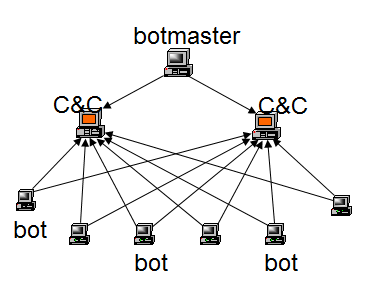
\includegraphics[width=\linewidth]{figures/botnet.png} \\ 
    Botnet Centralizzata
    \vspace{4ex}
  \end{minipage}%%
  \begin{minipage}[b]{0.5\linewidth}
    \centering
    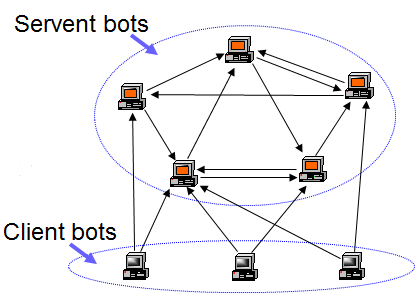
\includegraphics[width=\linewidth]{figures/botnetp2p.png} \\
    Botnet Decentralizzata 
    \vspace{4ex}
  \end{minipage} 
     \caption{Anatomia di Botnet\label{fig:botnet} }
\end{figure}

\subsection{Command and Control}
Durante la fase C\&C una macchina appena infettata diventa attivamente a far parte della botnet. Un bot tradizionale client-server, una volta installato su una nuova macchina, tenterà immediatamente il collegamento attraverso una rete IRC o contattando il server C\&C via HTTP.
I bot P2P decentralizzati ecentralised sono distribuiti con un metodo di bootstrapping predeficino per connettersi ad un DHT rilevante. Una volta connesse, le macchine compromesse chiedereanno ad uno deipropri peer riguardo gli ultimi comandi richiesti. Alcuni bot P2P richiedono che una specifica porta sia aperta ai peer per abilitare la comunicazione tra peer~\cite{p2pbots}. 
Vi sono due tecniche principali per la propagazione di comandi in un sistema botnet: push e pull.
In botnet basate su comunicazione IRC viene utilizzato il sistema push, in quanto i bot risiedono in una chat-room, in ascolto per nuovi comandi. 
In botnet basate su HTTP, i bot controllano periodicamente il server per verificare nuovi comandi. 
Reti basate su P2P possono agire in entrambe le modalità in quanto ricevono ed inviano comandi in maniera paritaria.


Molte famiglie di botnet contengono algoritmi di generazione di domini (DGA) per rendere le difese preventive inefficaci. I domini vengono generati algoritmicamente in maniera pseudo-randomica (decine di migliaia al giorno) da un campione iniziale. La macchina infetta successivamente invia una richiesta HTTP ad una larga parte di tali domini contemporaneamente, nella speranza che uno di questi domini sia effettivamente registrato e ospiti il C\&C della botnet. L'attacker ha solamente il compito di registrare un piccolo numero di questo domini, avendo a disposizione gli stessi domini generati. Dal lato dei difensori invece è necessario che tutti i domini generati da tali algoritmi siano rilevati e inseriti in una lista di esclusione per ottenere una difesa efficace della rete. Tale metodo di difesa risulta via via più inefficiente man mano che il numero d domini DGA aumenta.

\newpage
\section{Machine Learning}
\label{machinelearning}
Il Machine Learning è un sottocampo dell'intelligenza artificiale (IA) è stato definito da Arthur Samuel nel 1959~\cite{5392560}. L'obiettivo del machine learning generalmente è capire la struttura dei dati e adattare tali dati in modelli in grado di essere capiti e utilizzati da utenti.

Nonostante il Machine Learning sia un campo informatico, si differenzia dai tradizionali approcci computazionali. Nell'informatica tradizionale, gli algoritmi sono serie di istruzioni programmate esplicitamente usate dai calcolatori per elaborare dati o risolvere problemi. Gli algoritmi Machine Learning, al contrario, permettono ai calcolatori di allenarsi su input di dati ed usare analisi statistica in modo da produrre valori che ricadono all'interno di intorni specifici. Grazie a questo, il machine learning facilita ai calcolatori la costruzione di modelli che siano in grado di automatizzare processi decisionali basati su campioni di dati.

Molti campi tecnologici odierni sfruttano i benefici del machine learning; ad esempio tecnologie di riconoscimento facciale permettono alle piattaforme di social networks di aiutare gli utenti nel tag delle foto di amici. Altro esempio sono le tecnologie di Optical Character Recognition (OCR) in grado di convertire immagini di testi stampati in documenti testuali modificabili da un word processor. I recommendation engines, basati su machine learning, suggeriscono agli utenti i programmi televisivi o film basati sulle loro preferenze. Le auto a guida autonoma si basano su machine learning in molte applicazioni, ad esempio per il riconoscimento della segnaletica stradale.

Nel machine learning i compiti sono generalmente classificati in grandi categorie. Tali categorie sono basate su come l'apprendimento è impostato o su come il feedback dell'apprendimento viene dato al sistema.

Due dei metodi di apprendimento più comunemente adottati sono l'apprendimento supervisionato in cui si allenano algoritmi basandosi su input e output di esempio, categorizzati da esseri umani e l'apprendimento non supervisionato, in cui non vengono forniti dati categorizzati agli algoritmi in modo da permettere al sistema di trovare autonomamente la struttura che compone i dati di input. Nelle sezioni seguenti si mostrano tali metodi in dettaglio.

\subsection{Tipologie di Problemi}
Il machine learning è impiegato principalmente per la risoluzione di tre tipologie di problemi:
\begin{itemize}
\item \textbf{classificazione}, quando è necessario decidere a quale categoria appartiene un determinato dato. Ad esempio per l'identificazione di specie di piante fornendo un'immagine.
\item \textbf{raggruppamento} (clustering), quando si vuole raggruppare i dati che presentano caratteristiche simili. Ad esempio, un sistema può raggruppare immagini di figure geometriche separando figure con 4 lati e i cui angoli sono a 90 gradi oppure tutte le figure con quattro lati in cui solo due sono paralleli, ecc. In marketing, ad esempio, il raggruppamento viene utilizzato per l'individuazione di clienti e mercati potenziali.
\item \textbf{regressione}, cioè prevedere il valore futuro di un dato avendo noto il suo valore attuale. Un esempio è la previsione della quotazione delle valute o delle azioni di una società. Nel marketing viene utilizzato per prevedere il tasso di risposta di una campagna sulla base di un dato profilo di clienti; nell'ambito commerciale per stimare come varia il fatturato dell'azienda al mutare della strategia.
\end{itemize}

\subsection{Apprendimento Supervisionato}
Nell'apprendimento supervisionato, vengono forniti al sistema dei dati di input già etichettati con l'output desiderato. Lo scopo di tale metodo è permettere all'algoritmo di apprendimento di imparare comparando il suo output con quello fornito in ingresso, in modo da rilevare errori e modificare il modello di conseguenza. L'apprendimento supervisionato perciò usa patterns per predire i valori delle "etichette" su dati non etichettati.

Ad esempio, con l'apprendimento supervisionato, si può fornire ad un algoritmo un insieme di immagini di squali, etichettati come $pesce$ e immagini di oceani etichettati come $acqua$. Allenandosi su tali dati, l'algoritmo supervisionato dovrebbe essere in grado di riconoscere immagini di squali ed etichettarle come $pesci"$ ed immagini di oceani ed etichettarle come $acqua$.

Un comune uso dell'apprendimento supervisionato è l'uso di dati storici per predire probabili eventi futuri. Può usare informazioni statistiche sull'andamento del mercato azionario ed anticipare fluttuazioni future o utilizzato per filtrare email di spam. E' possibile utilizzare foto di cani etichettate per identificare la razza di un cane unicamente dalla sua foto.

\subsection{Apprendimento non Supervisionato}
Nell'apprendimento non supervisionato, i dati non sono etichettati. L'algoritmo viene lasciato libero di rilevare affinità tra i dati di input. Siccome i dati non classificati sono molto piu comuni che grandi quantità di dati etichettati, i metodi di machine learning che facilitano l'apprendimento non supervisionato sono considerabili come molto pregiati.

L'obiettivo dell'apprendimento non supervisionato può essere diretto, come la ricerca di pattern nascosti all'interno dei dati, ma può anche avere l'obiettivo di \textit{feature learning}: l'apprendimento di caratteristiche particolari che permette al sistema di scoprire automaticamente le rappresentazioni necessarie a classificare i dati grezzi.

L'apprendimento non supervisionato viene comunemente utilizzato per dati transazionali. Ad esempio, nel caso reale di un grosso dataset di clienti e dei loro acquisti, un essere umano difficilmente riuscirebbe a ricavare gli attributi che legano i profili clienti e le tipologie dei loro acquisti. Tuttavia fornendo tali dati ad un algoritmo di  apprendimento non supervisionato è possibile rilevare caratteristiche che legano determinati gruppi di clientela a determinati prodotti e di conseguenza prendere decisioni di marketing mirate.

L'apprendimento non supervisionato, grazie alla mancanza di un target da raggiungere, è in grado di analizzare dati che   apparentemente non mostrano relazioni ed estrarne dati significativi. Viene spesso usato per eseguire \textit{anomaly detection}, come l'utilizzo fraudolento di carte di credito; oppure è possibile eseguire classificazione di immagini (come nel precedente caso di razze canine) in maniera autonoma partendo da immagini non categorizzate.

\subsection{Apprendimento Semi Supervisionato}
Posto a metà tra il supervisonato e il non-supervisionato, l'apprendimento parzialmente supervisionato si basa su dati misti in cui una minima parte è già etichettata e una larghissima maggioranza è costituita da dati non etichettati.  Questo approccio viene utilizzato per migliorare le previsioni fatte dalla macchina sui dati non etichettati e richiede, normalmente, l'intervento di un analista. L'approccio è principalmente usato nei problemi di classificazione e di raggruppamento o nella descrizione delle relazioni causa-effetto tra le variabili.

\subsection{Apprendimento per Rinforzo}
L'apprendimento per rinforzo (Reinforcement learning) è una tecnica di apprendimento automatico che punta a realizzare sistemi in grado di apprendere ed adattarsi ai cambiamenti dell'ambiente in cui sono immersi attraverso la distribuzione di una “ricompensa” detta rinforzo, data dalla valutazione delle prestazioni.
Il suo funzionamento è attuato da tre componenti:
\begin{itemize}
\item un sistema logico di esecuzione (definito A), che sulla base dei dati in ingresso (Input) riesce a restituire un risultato (Output)
\item un sistema logico di valutazione (definito B) che assegna un premio (se il risultato è corretto) o una penalità (se il risultato non è corretto) al sistema logico A
\item un sistema logico di ottimizzazione (definito C) che osserva il comportamento di A e B e modifica il modello utilizzato da A per aumentare il premio e ridurre le penalità che B assegna ad A.
\end{itemize}

L'apprendimento per rinforzo è utilizzato in tutti quei campi in cui è essenziale che la macchina risponda ai cambiamenti dell'ambiente. Per questo è utilizzato frequentemente nella robotica, per controllare i movimenti degli automi, ma anche nelle auto a guida autonoma. Trova anche applicazione in ambiti industriali nella produzione e nel controllo qualità e in diversi altri settori.



\newpage
\section{Deep Learning e Reti neurali}
Il Deep Learning è uno specifico sottocampo del machine learning, un diverso modo di apprendere rappresentazioni di dati, principalmente orientato verso l'apprendimento di successivi strati (\textit{layers}) di rappresentazione via via più significativi. Il termine "deep" indica la presenza di questa moltitudine di strati che compongono il modello
di rappresentazione dei dati; infatti il deep learning odierno comprende generalmente modelli composti da decine o centinaia di strati successivi di rappresentazione, i quali apprendono in maniera automatica tramite l'esposizione ai dati di allenamento. Per confronto, gli approcci di machine learning descritti in sezione~\ref{machinelearning} generalmente coinvolgono uno o due strati di rappresentazione dei dati. Difatti tali modelli vengono definiti anche come \textit{shallow learning}.
 
\begin{figure}[htbp]
	\centering
	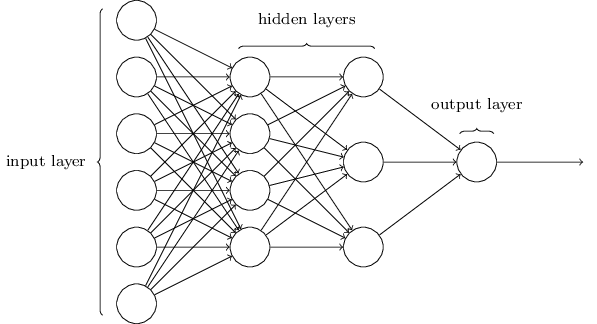
\includegraphics[width=\columnwidth]{figures/mlp-network.png}
	\caption{Schema generico di una rete Neurale \label{nn}}
\end{figure} 
 
All'interno del deep learning, queste rappresentazioni a più strati sono quasi unicamente apprese attraverso modelli definiti \textbf{reti neurali}, strutturati letteralmente in strati sovrapposti gli uni agli altri. Il termine "rete neurale" deriva dal campo della neurobiologia, tuttavia non si tratta di veri e propri modelli del funzionamento del cervello umano.

\begin{figure}[!bp]
	\centering
	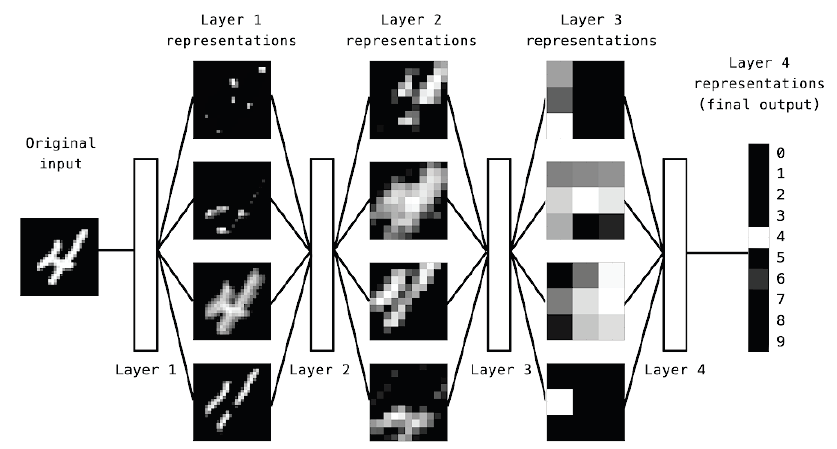
\includegraphics[width=\columnwidth]{figures/deeplearning.png}
	\caption{Esempio di rappresentazione di una cifra numerica tramite rete neurale. \textit{fonte}%
	~\cite{chollet2017deep} \label{fig:neuralnetwork} }
\end{figure}

Come è possibile vedere in figura~\ref{fig:neuralnetwork}, la rete neurale trasforma l'immagine di una cifra numerica disegnata a mano in una rappresentazione via via più informativa riguardo il risultato finale. Si può considerare il deep leraning come una operazione di distillazione di informazioni composta da più fasi in cui i dati vengono filtrati in maniera sempre più fine.

\subsection{Funzionamento Reti Neurali}
Le informazioni specifiche riguardo quali operazioni un livello apporta ai dati di input sono immagazzinate all'interno degli strati stessi, nella matrice dei "pesi". La trasformazione implementata da un livello è parametrizzata da tali pesi. Generalmente la fase di apprendimento consiste nel trovare un set di valori per i quali i pesi di tutti gli strati che compongono una rete neurale mappino correttamente i dati di esempio ai loro target associati.
Tuttavia l'operazione di ricerca dei valori ottimali non è triviale, in quanto una rete neurale può contenere fino a decine di milioni di parametri e rilevarne i valori corretti risulta in una operazione complessa.

Per superare tale vincolo, la fase di apprendimento di una rete neurale è composta da più fasi di osservazione, nel quale si misura quanto distante si trova l'output da quanto atteso. Tale è il compito della funzione di \textit{loss}. La funzione di loss utilizza la predizione della rete neurale e l'output atteso e computa un punteggio di distanza, catturando quindi la performance della rete sull'esempio analizzato.

Il meccanismo principale nel deep learning è l'uso di questo punteggio come segnale di \textit{feedback} per aggiustare il valore dei pesi in maniera da diminuire il valore del punteggio di loss per l'esempio analizzato. Questo aggiustamento è compito dell'\textit{ottimizzatore}, il quale implementa l'algoritmo di \textit{backpropagation} che attua la modifica dei pesi durante la fase di apprendimento.

Inizialmente i pesi della rete neurale sono assegnati a valori randomici, causando per le prime fasi di apprendimento un valore di loss particolarmente alto. Via via che le fasi di apprendimento mostrano diversi esempi alla rete i pesi vengono aggiustati di una piccola parte nella direzione corretta, causando una decrescita nel punteggo di loss. Questo \textit{training loop} viene ripetuto per un numero sufficiente di volte fino al raggiungimento di un valore minimo di loss e alla produzione di output il più possibile simile a quello desiderato. In figura~\ref{fig:neuralloss} è mostrato uno schema di alto livello.

\begin{figure}[!htbp]
	\centering
	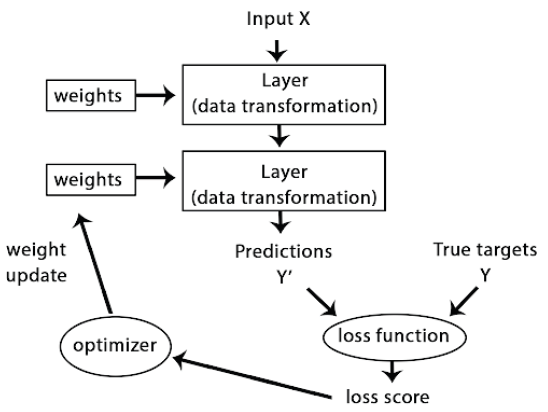
\includegraphics[width=0.8\columnwidth]{figures/deeploss.png}
	\caption{Schema di alto livello del funzionamento di una rete neurale. \textit{fonte}%
	~\cite{chollet2017deep} \label{fig:neuralloss} }
\end{figure}

\newpage
\section{Adversarial Learning}
Le tecniche di machine learning possono essere utilizzate per prevenire azioni vietate o illegali e nel caso vi siano degli incentivi economici, vi possono essere probabili antagonisti intenzionati ad eludere tali restrizioni. Un esempio tipico è il caso del filtraggio anti spam, nel quale gli spammers forgiano messaggi ad hoc per eludere le più recenti tecniche di filtraggio. Tali tecniche possono essere identificate come \textit{adversarial learning} (apprendimento antagonista).

Le vulnerabilità dei metodi di machine learning rispetto a manipolazione antagonista non possono venire semplicemente ignorate con la richiesta di tecniche più "robuste". I fondamenti teorici del machine learning odierno sono largamente costruiti sull'assunto che i dati di allenamento descrivano adeguatamente la realtà del fenomeno studiato. Questo assunto viene chiaramente violato nel caso che le distribuzioni di allenamento o di test vengano alterate, assumendo che gli antagonisti utilizzino qualsiasi mezzo possibile per disturbare l'algoritmo di apprendimento. I metodi di apprendimento in caso di ambienti antagonisti dovrebbero quindi essere in grado di sostenere una distorsione nei propri dati.

Come dimostrato da ricerche precedenti (~\cite{kearnsli},~\cite{Auer2002},~\cite{paclearning} ) un antagonista senza vincoli che può arbitrariamente alterare dati e target, può introdurre un errore fino al 100\%. Tuttavia nei casi pratici gli attackers devono atteneresi a determinati vincoli; ad esempio una email di spam deve recapitare il suo messaggio, un malware inviato ad un host deve eseguire correttamente e sfruttare una vulnerabilità e antagonisti che cercano di alterare i motori di ricerca possono controllare solo una frazione di tutti i domini raggiungibili. In alcuni casi si può mostrare come certi vincoli possono rendere la rilevazione di un attacco computazionalmente intrattabile~\cite{fogla}.

L'investigazione di metodi di machine learning per ambienti ostili è stata attuata in tre aree di ricerca largamente distinte: machine learning, sicurezza informatica e spam filtering. Nel caso di machine learning ricerche precedenti si sono incentrate su metodi di minimo-massimo con l'obiettivo di ottenere robustezza rispetto alla incertezza dell'input. Ad esempio classificatori più robusti sono stati sviluppati per gestire casi come il feature deletion~\cite{globerson} ; oppure ricerche hanno dimostrato che equilibri unici di Nash esistono per alcune tipologie di situazioni antagoniste~\cite{nash} .

Una differente visione dei problemi di apprendimento antagonista è emersa nel campo della sicurezza informatica, specialmente per quel che riguarda il rilevamento di intrusioni (\textit{intrusion detection} ). Diversi metodi sono stati proposti per rilevare pacchetti di rete anomali o per generare automaticamente \textit{signatures} strettamente legate a metodi di machine learning (ad esempio i lavori eseguiti in~\cite{wangstolfo} e~\cite{wang2006} ).

L'area dello spam filtering ha richiesto sforzi fondamentali da parte degli esperti in sicurezza; la costante ricerca di tecniche di evasione dei filtri anti-spam ha portato a studi estensivi riguardo vincoli e tecniche robuste di filtering~\cite{dalvi}. 

Il machine learning può fornire soluzione a difficili problemi di sicurezza di rete, compresi filtri anti-spam, rilevazione di vari tipologie di attacchi contro server e host, rilevazione di pagine web 
deliberatamente modificate per manipolare i motori di ricerca sfruttandone le vulnerabilità. Tutte queste problematiche riguardano la manipolazione di grandi quantità di dati in un ambiente altamente variabile e il bisogno di tecniche di classificazione veloci ed accurate. L'esistenza di antagonisti che possono trarre profitto in queste aree complica l'applicazione di machine learning e crea una "corsa agli armamenti" tra chi sviluppa classificatori sempre piu robusti e antagonisti che cercano di manipolare tali classificatori. Fortunatamente ogni area di applicazione fornisce vincoli riguardo le azioni antagoniste che rendono la classificazione fattibile. 

\begin{figure}[!htbp]
	\centering
	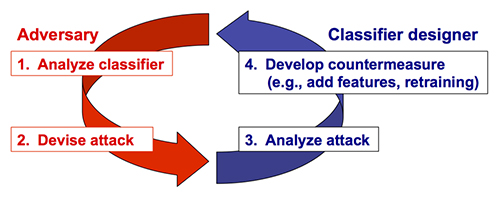
\includegraphics[width=\columnwidth]{figures/Reactive_arms_race.jpg}
	\caption{Schema concettuale del rapporto tra difensori ed antagonisti. \textit{fonte}%
	~\cite{wiki:Adversarial_machine_learning} \label{fig:advarms} }
\end{figure}

\newpage
\section{Generative Deep Learning}
I recenti risultati ottenuti nell'ambito del machine learning e del deep learning hanno permesso di ottenere algoritmi e architetture in grado di modellare complesse strutture di dati come immagini, suoni e testo. Questi avanzamenti sono stati incentrati principalmente in algoritmi di apprendimento supervisionato in grado di stimare una distribuzione di probabilità $p(x|y)$ dato un input ed un output di target. Tali modelli vengono definiti come modelli discriminativi o predditivi.

I modelli Generativi, al contrario, tentano di apprendere una funzione $p(y,x)$ nota come \textit{probabilità congiunta}. Tali funzioni di probabilità sono correlate secondo la relazione: 
\[p(x,y)=p(x)p(x|y)\]
dove $p(x)$ indica la densità di probabilità per l'evento $x$. 
Nel caso di modelli generativi, il modello ha accesso alla probabilità di input ed output allo stesso istante; permettendo ad esempio di generare immagini di animali, campionando specie di animali $y$ e nuove immagini $x$ a partire da $p(x,y)$.
Il passo successivo è l'abilità di apprendere solo la funzione di densità $p(x)$, dipendente unicamente dallo spazio degli input. Tali algoritmi sono definiti come Modelli Generativi non Supervisionati (\textit{Unsupervised Generative Models}), dove il termine \textit{generativo} indica l'abilità di campionare dalla distribuzione catturata dal modello. 

L'idea fondamentale alla base dei modelli generativi è la volontà di convertire il problema di generazione di dati in un problema di predizione ed usare l'insieme di tecniche di deep learning già note per risolvere tale problema. Gli algoritmi di deep learning odierni sono in grado di modellare mappature molto complesse e offrono flessibilità nel definire problemi in termini di grafi computazionali che possono essere ottimizzati da varianti di algoritmi di back-propagation.

\subsection{Autoencoder}
La forma più semplificata di conversione da problema generativo a problema discriminativo è l'apprendimento di una mappatura a partire dallo spazio degli input stesso. Sia dato un input $x$, si vuole ottenere una identità di tale input $x=f(x)$ dove $f$ rappresenta il modello predittivo. Il modello generativo può essere definito come l'insieme formato da un modello \textit{encoder} $q_e(h|x)$ in grado di mappare l'input in un nuovo spazio, definito come \textit{spazio latente} rappresentato da $h$ ed un modello \textit{decoder} $q_d(x|h)$ in grado di apprendere la mappatura inversa a partire dallo spazio latente.
Queste due componenti possono essere connesse assieme, a formare un modello end-to-end allenabile, caratterizzato da un vincolo di dimensione nello spazio latente $h$; generalmente definito come una riduzione di dimensione con lo scopo di far apprendere al modello un vettore di caratteristiche fondamentali dell'input. (figura~\ref{fig:aut}

\begin{figure}[!htbp]
	\centering
	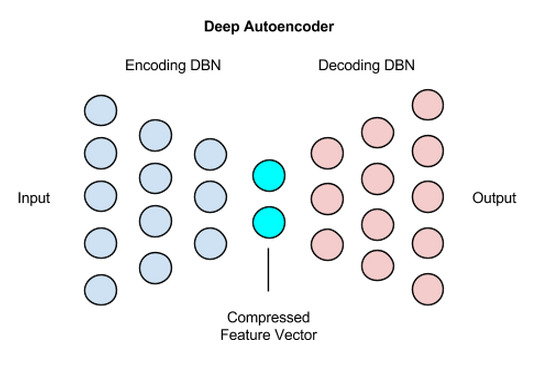
\includegraphics[width=\columnwidth]{figures/deep_autoencoder.png}
	\caption{Schema concettuale di un Autoencoder.  \label{fig:aut} }
\end{figure}

Una volta che il modello è stato appreso, decoder ed encoder possono essere utilizzati indipendentemente, ad esempio per generare nuovi campioni a partire dallo spazio latente.

\subsection{Generative Adversarial Networks}
La naturale evoluzione delle architetture Autoencoder è la Generative Adversarial Network in cui encoder e decoder vengono rimodellati due reti :discriminatore e generatore. 

Con l'obiettivo di apprendere la distribuzione del \textit{generatore} $p_g$ rispetto ai dati $\bm{x}$, si definisce precedentemente una variabile di rumore input  $p_{\b{z}}(\bm{z})$, e successivamente si rappresenta una mappatura dello spazio dei dati come $G(\bm{z}; \theta_g)$, dove $G$ è una funzione differenziabile rappresentata da una rete neurale a parametri $\theta_g$. Si definisce inoltre una seconda rete neurale \textit{discriminatore}
 $D(\bm{x}; \theta_d)$ che emette un singolo scalare. $D(\bm{x})$ rappresenta la probabilità che tale $\bm{x}$ provenga dai dati reali piuttosto che da $p_g$. 
A tal scopo si allena $D$ per massimizzare la probabilità di assegnare l'etichetta corretta sia ai campioni di allenamento che a quelli provenienti da $G$.
Simultaneamente si allema $G$ per minimizzare $\log(1-D(G(\bm{z})))$:

In altri termini, $D$ e $G$ eseguono una partita a due giocatori di minimo-massimo con funzione di valore $V(G, D)$: 

\begin{equation}
\label{eq:minimaxgame-definition}
\min_G \max_D V(D, G) = \mathbb{E}_{\bm{x} \sim p_{\text{data}}(\bm{x})}[\log D(\bm{x})] + \mathbb{E}_{\bm{z} \sim p_{\bm{z}}(\bm{z})}[\log (1 - D(G(\bm{z})))].
\end{equation}

In pratica è necessario implementare la partita in maniera iterativa. L'ottimizzazione di $D$ fino al completamento in un training a se stante risulta computazionalmente proibitivo e su dataset finiti risulta nel fenomeno di \textit{overfitting}. In maniera differente si alternano $k$ passi di ottimizzazione di $D$ ed un passo di ottimizzazione di $G$. Questo risulta nel mantenimento di $D$ vicino alla sua soluzione ottimale, cambiando gradualmente $G$. Questa strategia è mostrata formalmente all'interno dell'algoritmo~~\ref{alg:AGF}.

In pratica l'equazione~~\ref{eq:minimaxgame-definition} può non fornire un gradiente sufficiente per permettere a $G$ di apprendere. Nelle fasi iniziali dove $G$ è debole, $D$ può rifiutare i campioni con buona certezza in quanto chiaramente differenti dai dati di training. In tal caso, $\log ( 1- D(G(\bm{z})))$ satura. Piuttosto che allenare $G$ al fine di minimizzare $\log (1 - D(G(\bm{z})))$ si allena per massimizzare $\log D(G(\bm{z}))$. 
Questa funzione obiettivo risulta nello stesso punto fisso che forma la dinamica di $G$ and $D$ ma fornisce un gradiente molto più stabile nelle fasi iniziali.

In figura~\ref{fig:intuition} viene mostrata la fase di apprendimento di una GAN. Tale architettura è allenata aggiornando simultaneamente il gradiente della distribuzione discriminativa ($D$, linea blu tratteggiata) in modo che discrimini tra campioni della distribuzione generatrice di dati (linea nera tratteggata) $p_{\bm{x}}$ e i campioni provenienti dalla distribuzione del generatore $p_g$ (G) (linea verde).
La linea nera orizzontale da cui $\bm{z}$ è campionato è in questo caso uniforme; mentre la linea nera superiore è parte del dominio di $\bm{x}$. Le frecce indicano come la mappatura $\bm{x}=G(\bm{z})$ imponga una distribuzione non uniforme $p_g$ sui campioni trasformati. $G$ si contrae in regioni ad alta densità ed espande in regioni a bassa densità $p_g$. 
Di seguito la descrizione di quanto mostrato in figura~\ref{fig:intuition}
\begin{itemize}
\item (a) si considera una coppia avversaria prossima alla convergenza: $p_g$ è simile a $p_\text{data}$ e
$D$ è un classificatore parzialmente accurato.

\item (b) Nell'iterazione interna dell'algoritmo, $D$ è allenato a discriminare dati convergenti da:

\[D^*(\bm{x}) = 
\frac{
    p_\text{data}(\bm{x})
    }{
        p_\text{data}(\bm{x}) + p_g(\bm{x})}
\]

\item (c) dopo un aggiornamento a $G$, il gradiente di $D$ ha guidato $G(\bm{z})$ verso regioni dove sia più probabile che sia classificato come dato.

\item (d) dopo numerosi step di training se $G$ e $D$ hanno sufficiente capacità, raggiungono entrambi un punto in cui entrambi non possono migliorarsi a causa di \[p_g = p_\text{data}\] Il discriminatore non è in grado di differenziare tra le due distribuzioni. (ad esempio: $D(\bm{x}) = \frac{1}{2}$).
\end{itemize}

\begin{figure}[p] 
  \begin{minipage}[b]{0.5\linewidth}
    \centering
    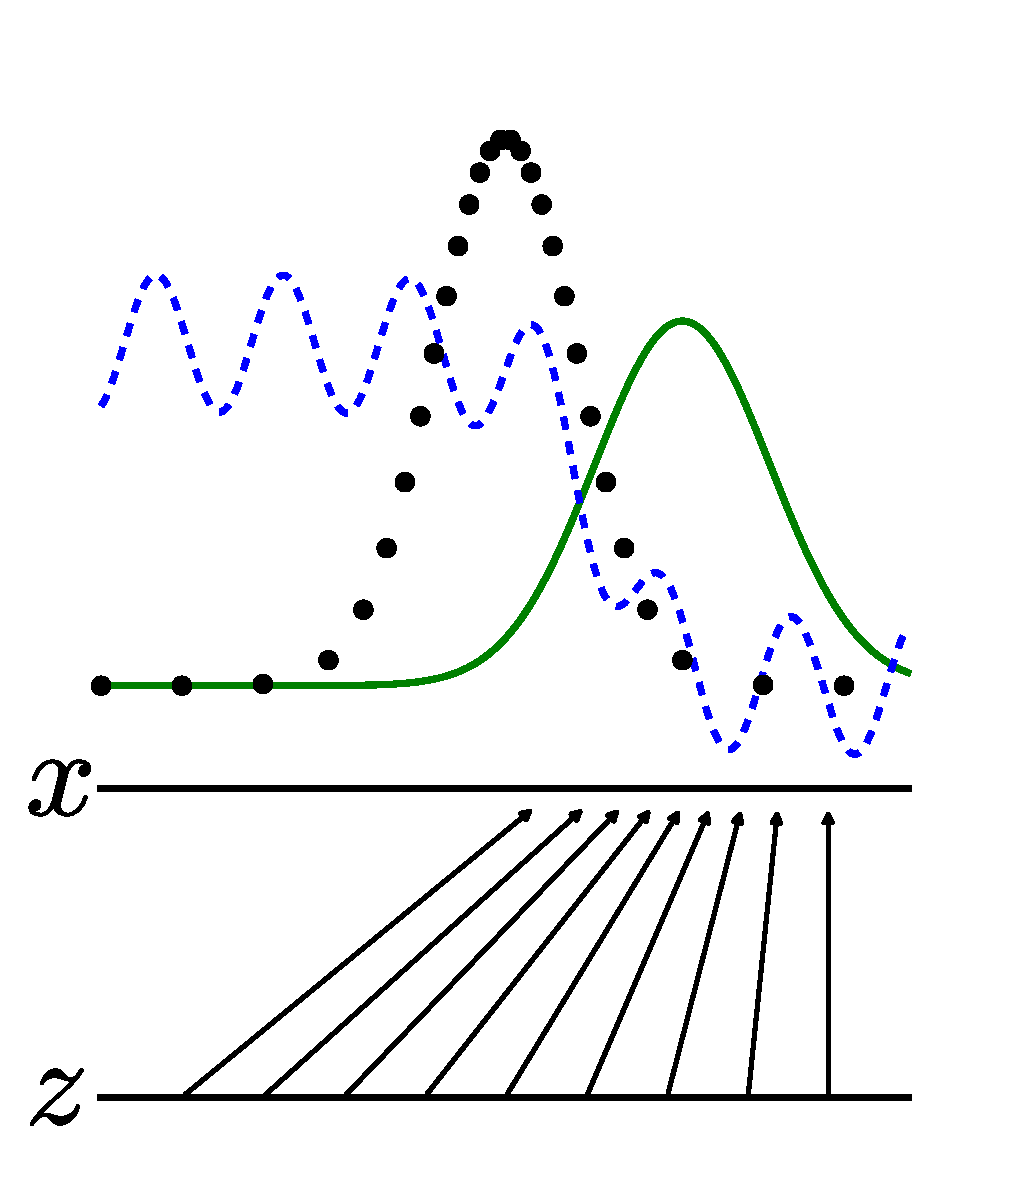
\includegraphics[width=.9\linewidth]{figures/fig1.pdf} \\ 
    (a)
    \vspace{4ex}
  \end{minipage}%%
  \begin{minipage}[b]{0.5\linewidth}
    \centering
    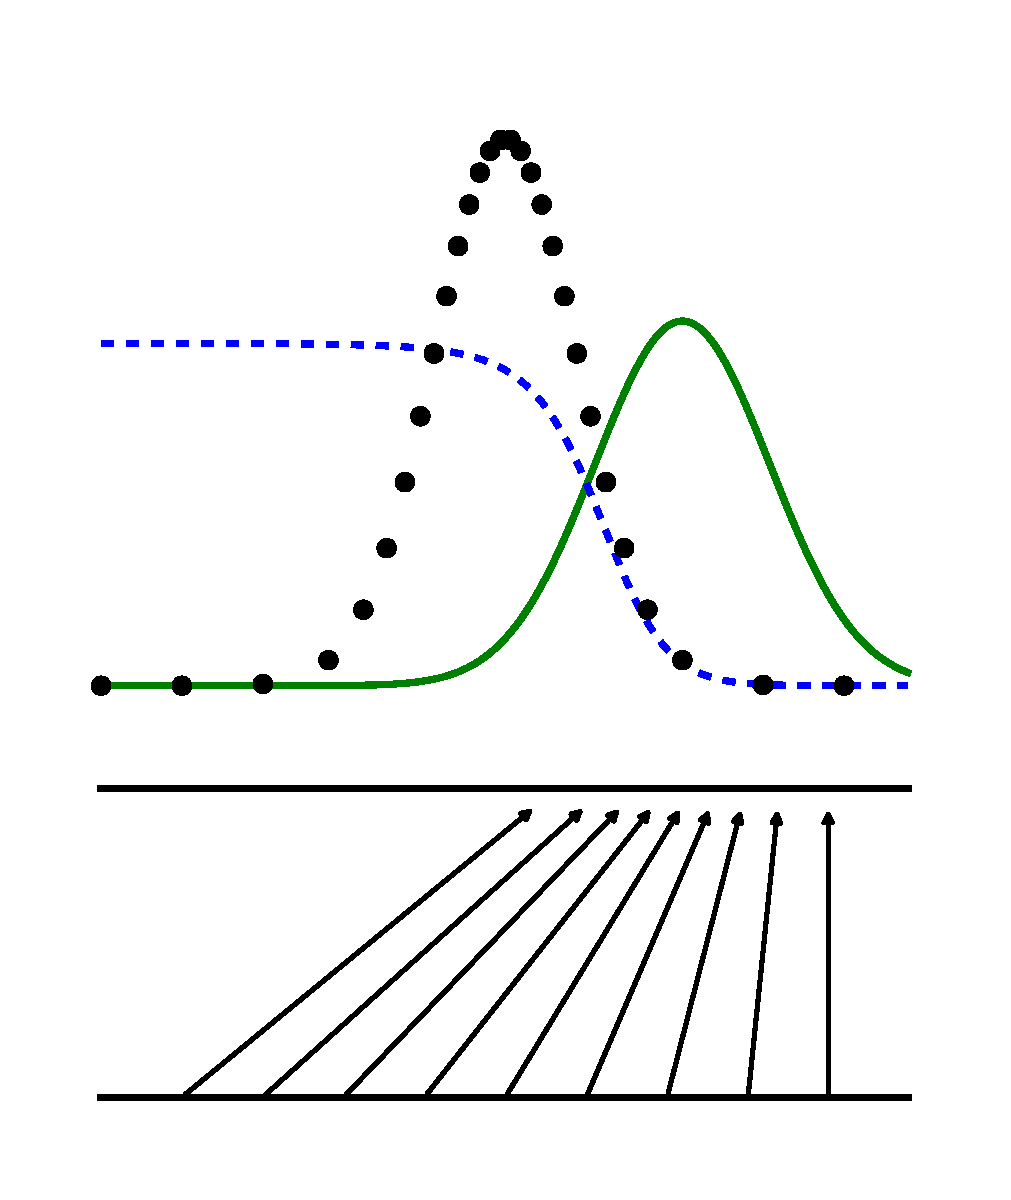
\includegraphics[width=.9\linewidth]{figures/fig2.pdf} \\
    (b) 
    \vspace{4ex}
  \end{minipage} 
  \begin{minipage}[b]{0.5\linewidth}
    \centering
    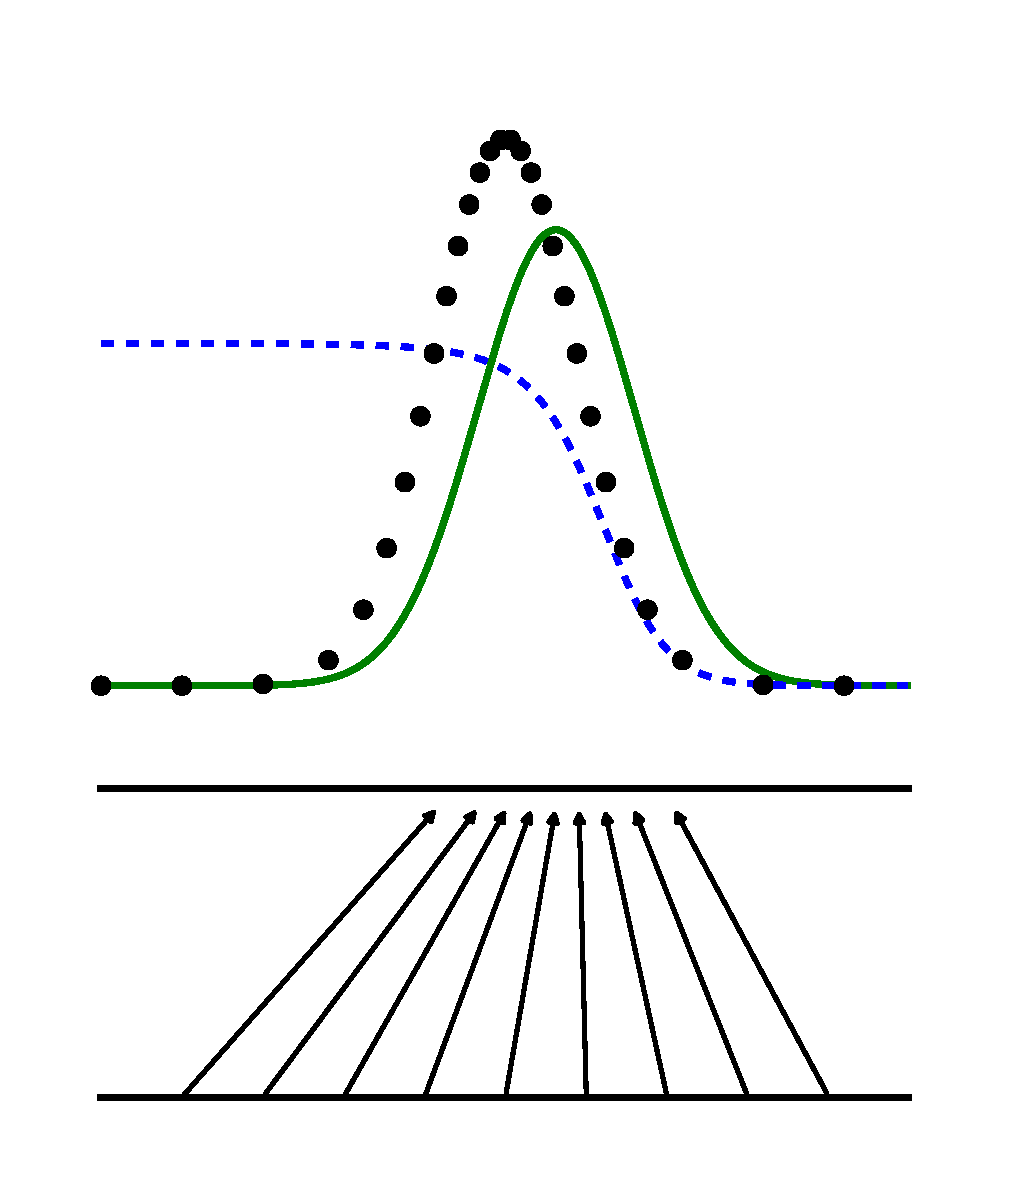
\includegraphics[width=.9\linewidth]{figures/fig3.pdf}  \\
    (c) 
    \vspace{4ex}
  \end{minipage}%% 
  \begin{minipage}[b]{0.5\linewidth}
    \centering
    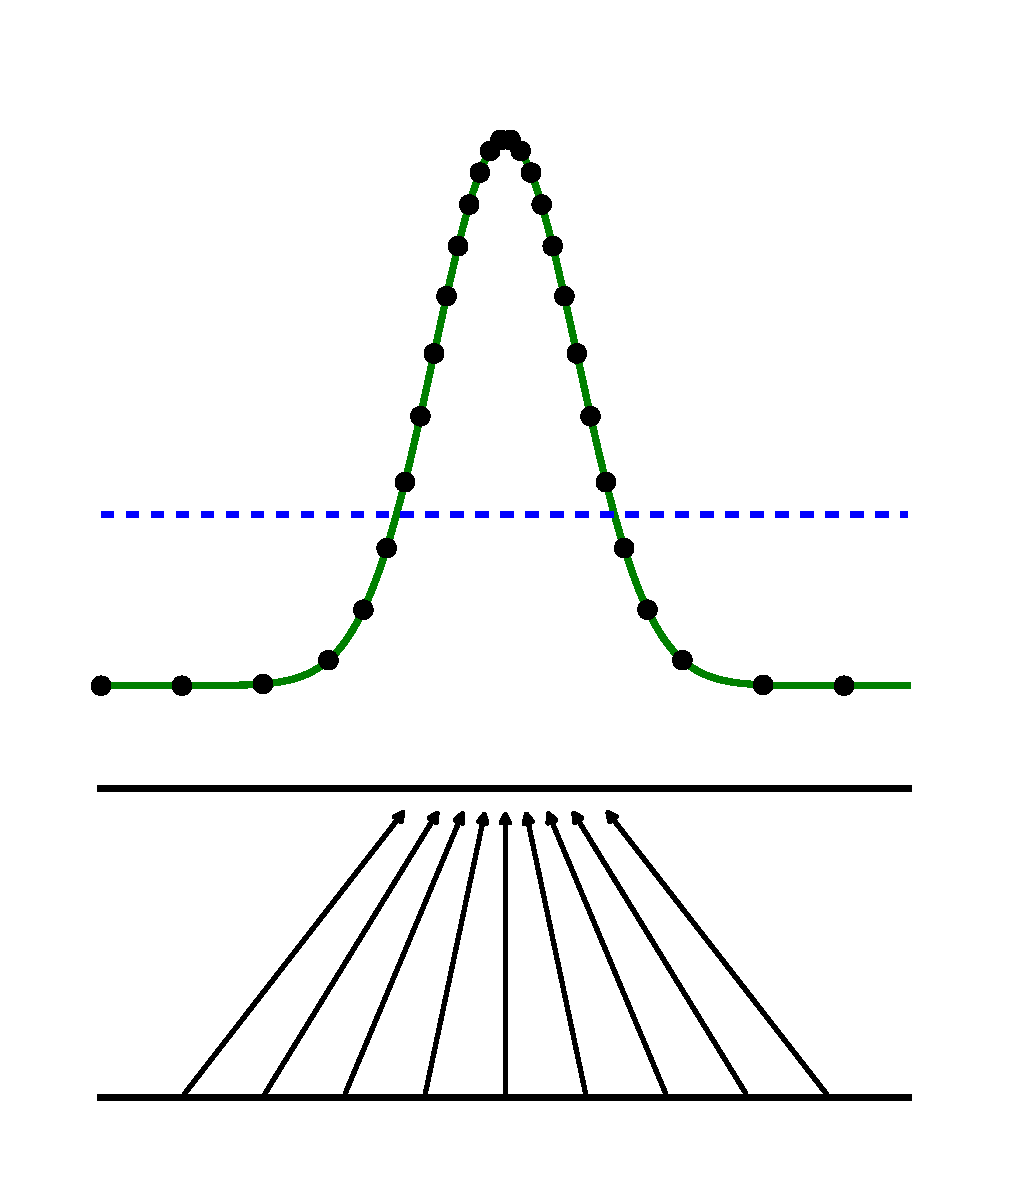
\includegraphics[width=.9\linewidth]{figures/fig4.pdf} \\
   (d) 
    \vspace{4ex}
  \end{minipage}
   \caption{\label{fig:intuition} }
 
\end{figure}

Il minimo globale del criterio di training virtuale $C(G)$ è ottenuto solo se $p_g=p_\text{data}$. 
A tal punto, si raggiungerà il valore $C(G) = -\log 4$. 
Se $G$ e $D$ hanno sufficiente capacità e ad ogni step dell'algoritmo~\ref{alg:AGF} il discriminatore è in grado di raggiungere il suo ottimo dato $G$, ed inoltre se $p_g$ venga aggiornato così da migliorare il criterio 
\[\mathbb{E}_{\bm{x} \sim p_\text{data}}[\log D^*_G(\bm{x})] + \mathbb{E}_{\bm{x} \sim p_g}[\log (1 - D^*_G(\bm{x}))]\] 
allora $p_g$ convergerà a $p_\text{data}$.

\subsubsection{Vantaggi e Svantaggi}
Questo framework moderno presenta vantaggie  e svantaggi relativi ai precedenti framework. Gli svantaggi primariamente sono che non esiste una esplicita rappresentazione di $p_g(\bm{x})$, e che $D$ deve essere ben sincronizzato con $G$ durante la fase di training (in particolare, $G$ non deve essere allenato troppo senza aggiornare $D$, in modo da evitare uno scenario degenerativo in cui $G$ collassa troppi valori di $\mathbf{z}$ verso lo stesso valore di $\mathbf{x}$ per ottenere abbastanza diversità da modellare $p_\text{data}$). 
I vantaggi rispetto a modelli alternativi come le Catene di Markov sono principalmente di tipo computazionale. I modelli antagonisti possono trarre un vantaggio statistico non dovendo aggiornare la rete generatrice con campioni di dati ma solamente tramite il flusso di gradiente che attraversa il discriminatore. Questo significa che le componenti dell'input non sono copiate direttamente nei parametri del generatore. Un ulteriore vantaggio delle reti antagoniste è la capacità di rappresentare distribuzioni molto nette mentre metodi alternativi basati su Catene di Markov richiedono che la distribuzione sia meno distinta in modo da garantire alle catene la capacità di mischiare le modalità.

\begin{algorithm}[p]
\caption{Discesa stocastica del gradiente durante la fase di training di una GAN.
il numero di passi applicati al discriminatore, $k$, è un iperparametro della rete.
}
\begin{algorithmic}
\label{alg:AGF}
\FOR{numero di iterazioni di trainingons}
  \FOR{$k$ passi}
    \STATE{$\bullet$ Campionare un mini-batch di $m$ campioni generati da rumore $\{ \bm{z}^{(1)}, \dots, \bm{z}^{(m)} \}$ dal rumore precedente $p_g(\bm{z})$.}
    \STATE{$\bullet$ Campionare un mini-batch di $m$ esempi $\{ \bm{x}^{(1)}, \dots, \bm{x}^{(m)} \}$ dalla distribuzione di dati reali $p_\text{data}(\bm{x})$.}
    \STATE{$\bullet$ Aggiornare il discriminatore aumentando il proprio gradiente stocastico:
        \[
            \nabla_{\theta_d} \frac{1}{m} \sum_{i=1}^m \left[
            \log D\left(\bm{x}^{(i)}\right)
            + \log \left(1-D\left(G\left(\bm{z}^{(i)}\right)\right)\right)
            \right].
        \]}
    %parameters $\theta_d$ of discriminator $D$
   %in the direction of the stochastic gradient of the binomial cross-entropy
   %for $D$ predicting whether its argument comes from $p_\text{data}(\bm{x})$ (target = 1, input = $\bm{x}$) or
   %$P_g$ (target = 0, input = $G(\bm{z})$), i.e., towards minimizing
   % \mbox{$-\log D(\bm{x}) - \log(1 - D(G(\bm{z})))$}.}
   \ENDFOR
  \STATE{$\bullet$ Campionare un mini-batch di $m$ campioni generati da rumore $\{ \bm{z}^{(1)}, \dots, \bm{z}^{(m)} \}$ dal rumore precedente $p_g(\bm{z})$.}
    \STATE{$\bullet$ Aggiornare il generatore, aumentando il proprio gradiente stocastico:
        \[
            \nabla_{\theta_g} \frac{1}{m} \sum_{i=1}^m
            \log \left(1-D\left(G\left(\bm{z}^{(i)}\right)\right)\right)
            .
        \]}
  \ENDFOR
  \\Gli aggiornamenti di gradiente possono utilizzare qualsiasi legge di apprendimento.
  \end{algorithmic}
\end{algorithm}




\chapter{Progetto}
\label{progetto}

In questo capitolo si propone il progetto realizzato per raggiungere gli obiettivi preposti: la realizzazione di un classificatore basato sull'algoritmo di machine learning \textit{Random Forest} in grado di distinguere domini generati algoritmicamente da domini reali. Si è successivamente progettato un classificatore più raffinato basato su rete neurale che superasse le precedenti mancanze. Il passo successivo ha riguardato la creazione di una \textit{Generative Adversarial Network} basata sul progetto di un \textit{Autoencoder} in grado di generare domini sintetici realistici col fine di rafforzare il classificatore neurale.

\begin{figure}[htb]
    \centering
	%\documentclass{standalone}
%\usepackage{tikz}

%\usetikzlibrary{shapes,arrows,fit,calc,positioning}
%\usetikzlibrary{backgrounds}
\tikzstyle{input} = [coordinate]
\tikzstyle{output} = [coordinate]
\tikzstyle{box} = [draw, rectangle, fill=white, rounded corners, thick, node distance=10em, text width=7em, text centered, minimum height=5em]
\tikzstyle{container} = [draw, rectangle, dashed, inner sep=1em, node distance=5em]
\tikzstyle{line} = [draw, thick, -latex']
%\begin{document}
\begin{tikzpicture}[auto, node distance=10em]
	\node [input](input){};
	\node [box, right of=input](clas){Classificatore};
	\node [box, below of=clas](gan){Generative Adversarial Network};
	\node [container, fit=(gan)](adv){};
	\node at (adv.south) [below,node distance=0 and 0] {Adversarial Learning};	
	\node [output, right of=clas](output){};
		
	
	\path [line] (input) -- node[near start](dataset){Dataset} (clas);
	\path [line] (dataset) |- (gan);
	\path [line] (gan) -- node[right]{Rinforzo} (clas);
	\path [line] (clas) -- (output)node[near end,name=out]{Decisione};
\end{tikzpicture}
%\end{document}
\label{fig:intro}
\caption{Diagramma di progetto}
\end{figure}

\todo{schema da autoencoder a GAN}

\section{Classificatore Random Forest}
\label{randomforest}
La prima fase di questo studio è stata quella di implementare un classificatore in grado di separare efficacemente domini \textit{DGA} da domini reali basandosi unicamente sulle caratteristiche linguistiche dei domini: infatti, ad un esame preliminare, i domini \textit{DGA} presentano caratteristiche ben differenti da semplici frasi o parole che solitamente compongono i domini reali.

Si è scelto di utilizzare Random Forest in quanto ritenuto il più adatto al caso in esame. L'algoritmo è stato inoltre messo a confronto con \textit{Support Vector Machine} e \textit{Naive-Bayes}. \todo{indicare SVM e GNB solo nei risultati?}

All'interno del classificatore \textit{Random Forest} \cite{randomforest}, ogni albero dell'insieme è costruito a partire da un campione estratto con sostituzione dal \textit{training set}. In aggiunta, al momento della divisione del nodo durante la costruzione di un albero, la divisione scelta non è più la migliore soluzione tra tutte le \textit{features}. Al suo posto, la divisone che viene scelta è la migliore divisione all'interno di un \textit{subset} casuale tra tutte le \textit{features}. Come risultato di questa casualità, il \textit{bias} della foresta di solito aumenta leggermente (rispetto al \textit{bias} di un singolo albero non casuale) ma, a causa della media, la sua varianza diminuisce, di solito compensando l'aumento di \textit{bias}, quindi dando un modello generale migliore.

\subsection{Dataset}
\label{randomforestdataset}
I \textit{dataset} di \textit{training} e \textit{testing} sono stati ricavati due fonti differenti: per quel che riguarda i domini reali si è fatto riferimento alla classifica dei domini più visitati al mondo fornita da \textit{Alexa Internet Inc.} \cite{amazon:alexa} , per un totale di 1 milione di siti realmente esistenti; mentre grazie al repository fornito da \cite{github:dgarepo} è stato possibile ottenere un \textit{dataset} esaustivo di esempi \textit{DGA} da diverse famiglie di \textit{malware} tra i quali ransomware come \textit{cryptolocker} e \textit{cryptowall}, trojans bancari come \textit{hesperbot}, e information stealers come \textit{ramnit}. Le tecniche DGA tradizionali variano in complessità da semplici approcci che estraggono caratteri casualmente a quelli che cercano di mimare la distribuzione di lettere o parole trovate nei domini reali. Il DGA di \textit{ramnit}, ad esempio, crea nomi di dominio usando una combinazione di moltiplicazioni, divisioni e resti a partire da un seme randomico. Agli antpodi, \textit{suppobox} crea domini concatenando due parole scelte in maniera pseudo-casuale da un piccolo dizionario Inglese.
In tabella \ref{tab:dga} vengono mostrati alcuni esempi di domini generati algoritmicamente a seconda delle diverse famiglie di malware.
La maggior parte dei DGA opera a livello di singoli caratteri, mentre altre tipologie comuni come beebone hanno una struttura rigida, che produce domini come ns1.backdates13.biz e ns1.backdates0.biz.
Il DGA symmi produce domini vagamente pronunciabili tra i quali “hakeshoubar.ddns.net” estraendo una vocale o una consonante casualmente per ogni indice pari e successivamente estraendo l’opposto all’indice successivo oltre che ad aggiungere un dominio di primo e secondo livello al termine della stringe come .ddns.net
La distribuzione dei singoli caratteri (unigrammi) per 4 famiglie di DGA e Alexa sono mostrate di seguito. La distribuzione di cryptolocker e ramnit sono entrambe uniformi all’interno dello stesso range. Si tratta di una caratteristica attesa in quanto entrambi sono generati tramite una serie di moltiplicazioni, divisioni e resti basati su di un singolo seme. Suppobox, d’altro canto presenta caratteristiche interessanti in quanto genera unigrammi simili per distribuzione ad Alexa. 

\begin{table}[H]
    \centering
    \resizebox{0.4\textwidth}{!}{%
    \begin{tabular}{ l|l }
        corebot & ep16g6gjwfixyhs8gfy.ddns.net \\
 		& ev5texifc43nebil3pk.ddns.net \\
 		& gf7bm4163fmjkje.ddns.net \\
		cryptolocker & agryjvdaabkyt.ru \\
 		& pwitjnqgjfaqm.org \\
 		& dhhubfepcdgfv.co.uk \\ 
		dircrypt & hedhryendqlss.com \\
 		& lgnggnlufbtyjpnvct.com \\
 		& tzrbdmhoumoy.com \\
		kraken v2 & fwulvdmdytm.com \\
 		& gybuisybe.cc \\
 		& gyinkvye.net \\
		lockyv2 & btlwubflhfllshn.info \\
 		& cpgcjsysfwuwa.click \\
 		& jlbroeji.biz \\
		pykspa & gqjgflhop.net \\
 		& gqumcwaa.org \\
 		& jpivjh.net \\
		qakbot & fgfifkyfut.info \\
 		& flzuzsaekkipatbtet.biz \\
 		& owpbsjekk.com \\
		ramdo & kugmywaaiymaegiq.org \\
 		& ocywskaagmmqscoc.org \\
 		& uomywsaaqggiwouo.org \\
		ramnit & byqdmekgd.com \\
 		& dpmdbwwcmpk.com \\
 		& gkkcoufektvhiqr.com \\
		simda & gatyfusyfi.com \\
		& lyvyxoryco.com \\
 		& puvyxilomo.com \\
    \end{tabular}
    }
\label{tab:dga}
\caption{Esempi di domini generati algoritmicamente da Malware}
\end{table}


A partire da tale \textit{dataset} combinato si è proceduto alla creazione di un classificatore binario che fosse in grado di distinguere domini reali da domini generati algoritmicamente. 
Il passo seguente  stato creare una serie di \textit{features} che fossero in grado di descrivere le caratteristiche linguistiche dei domini presi in esame.


\begin{figure}[htb]
    \centering
    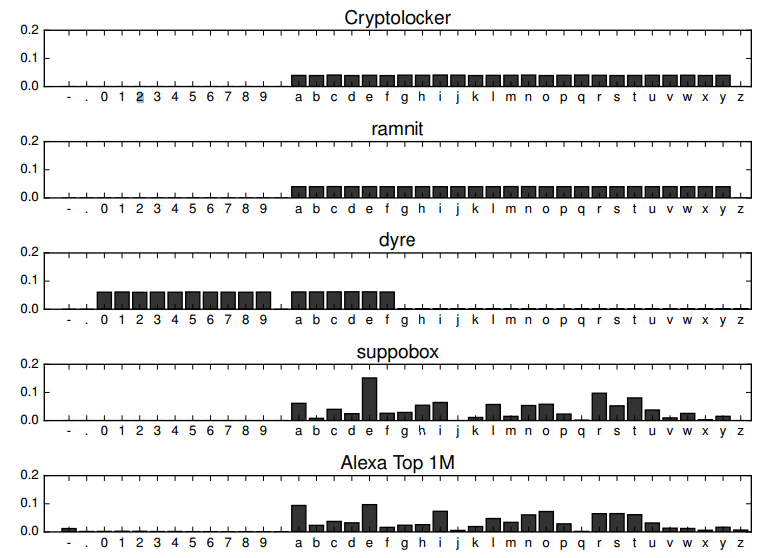
\includegraphics[width=0.8\columnwidth]{figures/chardistr.png}
    \caption{Distribuzione dei singoli caratteri in \textit{cryptolocker, ramnit, dyre}, \textit{suppobox} (dictionary-based DGA) ed il primo milione di domini più visitati secondo Alexa \cite{amazon:alexa}.
\textit{fonte:} \cite{deepdga}}
\label{fig:relu}
\end{figure}


Per raggiungere tale obiettivo si è fatto riferimento a ricerche già esistenti: \cite{180232} \cite{Yadav:2010:DAG:1879141.1879148} \cite{Yadav:2012:DAG:2428696.2428722} \cite{Schiavoni2014}. Di seguito viene illustrato l'insieme di tali \textit{features}:

\subsection{Features}
\label{randomforestinterno}

\begin{itemize}

\item \textbf{Rapporto tra caratteri significativi}. Modella il rapporto dei caratteri della stringa $p$ che formano una parola significativa all'interno del dizionario Inglese. Un valore basso indica la presenza di algoritmi automatici. In dettaglio, si divide $p$ in $n$ sotto-parole significative $w_i$ di almeno $3$ caratteri: $|wi| \ge 3$ cercando di lasciare fuori meno caratteri possibili: 

\[R(d) = R(p) = \frac{max(\sum_{i=1}^n |wi|)}{\left | p \right |}\] 

Se $p = \text{facebook}$, $R(p) = \frac{(|\text{face}| + |\text{book}|)}{8} = 1$ allora il dominio è composto completamente da parole significative, mentre $p = \text{pub03str}$, $R(p) = \frac{|\text{pub}|}{8} = 0.375$. 

    

\item \textbf{Punteggio di normalità degli n-grammi}: Questa classe di \textit{features} modella la pronunciabilità di un nome di dominio rispetto la lingua Inglese. Più la combinazione di fonemi del dominio è presente  all'interno del Dizionario Inglese più tale dominio è pronunciabile. Domini con un basso numero di tali combinazioni sono probabilmente generati algoritmicamente. Il calcolo avviene estraendo lo n-gramma di $p$ di lunghezza $n \in \left \{1, 2, 3, 4, 5 \right \}$ e contando il numero di occorrenze di tale n-gramma all'interno del Dizionario Inglese. Tali \textit{features} sono quindi parametriche rispetto ad n:
 
\[S_n(d) = S_n(p) \:= \frac{\sum_{\text{n-gramma t in p}} count(t)}{\left | p \right | - n + 1}\] 

dove $count(t)$ sono le occorrenze dello n-gramma nel dizionario. Ad esempio $S_2(facebook) = fa_{109} + ac_{343} + ce_{438} + eb_{29} + bo_{118} + oo_{114} + ok_{45} = 170.8$

       
\item \textbf{Rapporto tra caratteri numerici} Questa \textit{feature} rappresenta il rapporto tra i caratteri numerici presenti all'interno del nome di dominio rispetto la lunghezza totale della parola. Molte famiglie di \textit{malware} utilizzano \textit{DGA} che generano domini tramite una distribuzione uniforme di caratteri alfabetici minuscoli e numeri, questo porta a domini generati algoritmicamente che presentano una maggior presenza di numeri al loro interno rispetto ai domini reali.


\item \textbf{Rapporto tra vocali e consonanti} Questa \textit{feature} modella il rapporto tra vocali e consonanti all'interno del nome di dominio.


\item \textbf{Lunghezza del nome di dominio} Questa \textit{feature} calcola la lunghezza del dominio. Molte famiglie di \textit{malware} utilizzano \textit{DGA} che generano domini di lunghezza costante, generalmente molto lunghi rispetto ai domini reali.
	
\end{itemize}

L'implementazione di tali \textit{features} ha permesso di ottenere un \textit{dataset} in grado di modellare le caratteristiche linguistiche dei nomi di dominio mostrati al capitolo \ref{randomforestdataset}. Da tale spunto è partita la fase iniziale di \textit{testing} 

\subsection{Output}
\label{randomforestoutput}
L'obiettivo di tale classificatore è quello di riuscire a separare in maniera efficace i domini reali da quelli generati algoritmicamente. A tale proposito ???
\todo{ampliare questa sezione?}
\todo{indicare il capitolo coi risultati di Random Forest} 

Durante la fase di sperimentazione il classificatore si è rivelato efficace rispetto la maggior parte delle famiglie di \textit{DGA}. Il caso particolare della famiglia \textit{suppobox} \cite{geffner2013end} ha messo in particolare difficoltà il classificatore in quanto tale algoritmo genera domini in maniera pseudo-casuale, concatenando due parole a partire da un \textit{subset} del dizionario inglese di 384 parole. Tale caratteristica fa si che le \textit{features} linguistiche estratte da questa famiglia di \textit{malware} siano molto simili a quelle presenti nei domini reali. In tabella \ref{tab:suppobox} sono mostrati alcuni esempi di domini generati da Suppobox.


\begin{table}[htb]
    \centering
    \begin{tabular}{|l|}
        \hline
        Suppobox
        \\
        \hline
        \hline
       	increaseinside.net \\
		wouldinstead.net \\
		rememberinstead.net \\
		wouldexplain.net \\
		rememberexplain.net \\
		wouldbright.net \\
		rememberbright.net \\
		wouldinside.net \\
		rememberinside.net \\
        \hline
    \end{tabular}
    \caption{Esempio di domini generati da Suppobox.}
\label{tab:suppobox}
\end{table}

A partire da questo risultato si scelto di procedere con la progettazione di un classificatore neurale in grado di superare tale problematica.


\section{Classificatore Neurale}
\label{classificatorenn}
Questo classificatore neurale nasce con l'intento di superare le difficoltà incontrate dal precedente classificatore basato su \textit{Random Forest}, utilizzando le caratteristiche delle reti neurali, in grado di estrarre \textit{features} a partire dai dati grezzi. Si è scelto di partire dall'architettura di tipo \textit{Multilayer Perceptron} con l'obiettivo di ottenere risultati migliori rispetto al caso mostrato nella sezione precedente.

I passi del progetto sono stati la codificazione dei domini in valori numerici, l'individuazione di una architettura ottimale per classificare i dati in esame ed un'ultima fase di \textit{tuning} degli iperparametri della rete neurale. 

\subsection{Input}
\label{classificatorenninput}
A partire dal \textit{dataset} creato per il precedente caso, si è deciso di convertire direttamente i nomi di dominio alfanumerici in vettori numerici, mappati secondo il dizionario di tutti i caratteri ammessi \cite{icann} (lettere minuscole a-z, numeri 0-9, tratto d'unione "-" ). L'obiettivo è quello di fornire al classificatore neurale in questione una rappresentazione il più possibile aderente ai dati reali, senza l'ausilio di \textit{features} ingegnerizzate a priori, lasciando così la libertà alla rete neurale di estrarre le caratteristiche più appropriate per la distinzione dei domini. Come scelta progettuale si è deciso di limitare la dimensione dei domini a 15 caratteri per ognuno, in modo da ottenere un \textit{dataset} di dimensioni fissate e sopperire alle differenti lunghezze di ogni dominio tramite un semplice \textit{padding} di zeri in testa ad ogni stringa codificata.

Assieme ai dati codificati è stato generato un vettore di \textit{target} nel quale viene indicato da 0 o da 1 se il dominio in esame è di tipo reale o generato algoritmicamente. L'obiettivo quindi è di attuare un classificatore binario in grado di prevedere correttamente a quale categoria appartiene un dominio esaminato 

\subsection{Architettura Classificatore Neurale}
\label{classificatorenninterno}
L'architettura scelta in prima fase è stata quella del \textit{Multilayer Perceptron} \textit{(abbr. MLP)}, una tipologia di rete neurale \textit{feedforward} tipicamente formata da almeno tre livelli di nodi. Ad esclusione del livello di \textit{input} i livelli del MLP utilizzano  funzioni di attivazione non lineari che permettono di eseguire distinzioni tra dati non linearmente separabili. Considerando una rete formata da $m$ neuroni,  se si considera $d$ come numero di input, si avrà il seguente output

\[y_j=y\left( \sum_{i=0}^d w_{ji}x_i \right)\]


nel quale $x_i$ sono gli input e $w_{ji}$ sono i pesi di ogni input combinati con ogni output. 

Nel caso in esame è stata utilizzata per i livelli interni la funzione di attivazione \textit{Rectifier Linear Unit} (ReLU) \cite{relu} definita dalla funzione sottostante e mostrato in figura \ref{fig:relu}

\[f(x) = x^+ = max(0,x)\]

\begin{figure}[htb]
    \centering
    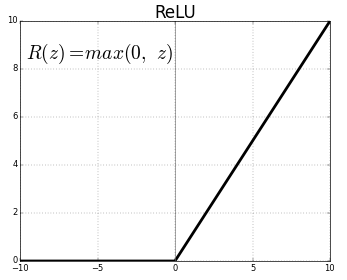
\includegraphics[width=0.5\columnwidth]{figures/relu.png}
    \caption{\textit{fonte:} \cite{relufig}}
\label{fig:relu}
\end{figure}

dove $x$ rappresenta l'\textit{input} del neurone. 
I vantaggi di tale funzione sono una migliorata \textit{performance} rispetto ad altre funzioni similari come \textit{tanh} e \textit{sigmoid} per quel che riguarda la convergenza della discesa stocastica del gradiente. 

Per quel che riguarda la funzione di attivazione del livello di \textit{output} si è scelta la funzione \textit{sigmoidea}, definita dalla formula 

\[P(t) = \frac{1}{1+e^{-t}}\]

\begin{figure}[htb]
    \centering
    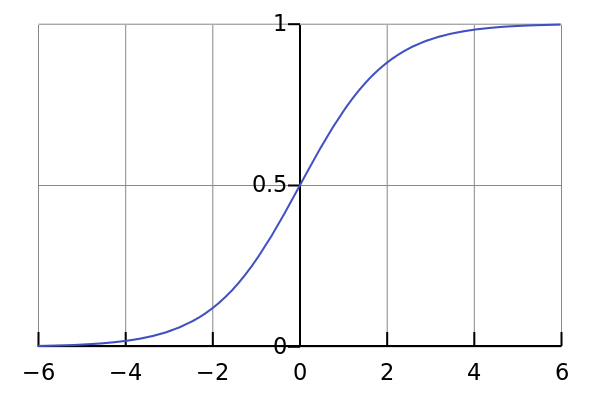
\includegraphics[width=0.5\columnwidth]{figures/sigmoid.png}
    \caption{\textit{fonte:} \cite{fig:sigmoid}}
\label{fig:sigmoid}
\end{figure}

La struttura finale del \textit{MLP} in esame è stata raggiunta dopo una serie di test sperimentali in cui si sono messi a confronto tre modelli differenti di per numero di neuroni all'interno degli \textit{hidden layer}: 
\begin{itemize}
\item un modello ridotto composto da un layer di input con un numero di neuroni pari alla dimensione delle stringhe codificate, un layer intermedio di dimensione dimezzata rispetto al precedente ed il layer finale di uscita di dimensione 1 per attuare la classificazione binaria, oggetto di studio.

\item un modello allargato composto da un layer di input con un numero di neuroni pari alla dimensione delle stringhe codificate, due layer intermedi di dimensioni moltiplicate di diversi ordini rispetto al layer iniziale ed un layer finale di dimensione 1.

\item un modello intermedio composto da un layer di input con un numero di neuroni pari alla dimensione delle stringhe codificate, un layer intermedio di dimensione 128, un layer di dimensione minore a 64 ed un layer finale di dimensione 1. (Figura \ref{fig:pieraz})

\end{itemize}

I tre modelli messi a confronto hanno mostrato risultati simili, tuttavia  il modello intermedio si è dimostrato più performante, con un costo computazionale irrisorio rispetto al modello allargato, pertanto è stato scelto come riferimento per gli studi successivi.

\begin{figure}[!htb]
    \centering
    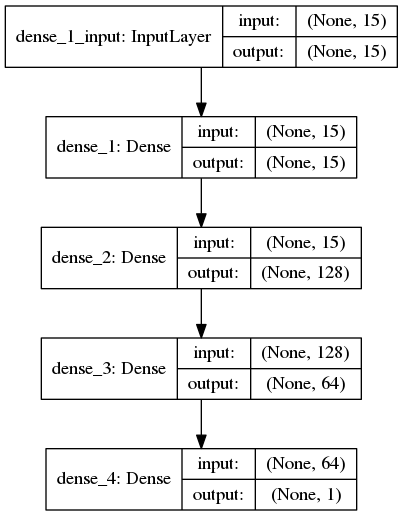
\includegraphics[width=.6\columnwidth]{figures/pieraz_baseline.png}
    \caption{Grafico del modello intermedio. Escluso il layer di input iniziale, si notino gli \textit{hidden layer} dense2 e dense3 di dimensioni rispettivamente 128 e 64 }
\label{fig:pieraz}
\end{figure}

\subsection{Output}
\label{classificatorennoutput}
L'intento della rete neurale proposta è quello di classificare autonomamente domini reali da domini generati algoritmicamente, con l'obiettivo di superare le fragilità del classificatore precedente (\ref{randomforest}) ed avere una linea di confronto affidabile per lo \textit{step} di lavoro successivo: l'introduzione di un sistema di \textit{adversarial learning} che possa rafforzare tale classificatore. 
\todo{come ampliare??????????????}

\section{Realizzazione Adversarial Learning}
\label{adv}
Ricerche precedenti hanno dimostrato che molti modelli di machine learning, incluse le reti neurali, sono vulnerabili agli \textit{adversarial examples} \cite{1312.6199},  \cite{1412.6572}. In particolare la ricerca proposta in \cite{1412.6572} introduce il metodo del \textit{fast gradient sign} per scoprire \textit{adversarial examples} perturbando un campione noto $x$ con una piccola quantità $\Delta x =  \in sign(\nabla_x J(\theta,x,y))$ dove $\theta$ rappresenta i parametri del modello e $J$ il costo necessario a classificare $x$ come $y$.
Separatamente \cite{1406.2661} propone l'uso di \textit{Generative Adversarial Network (abbr. GAN})  come \textit{framework} in grado di generare campioni artificiali provenienti dalla stessa distribuzione del training set.
Le \textit{GAN} incorporano due modelli: un generatore ed un discriminatore i quali competono in una serie di turni antagonisti. All'interno del contesto del lavoro presentato in questo elaborato, il generatore impara a creare nuovi domini artificiali mentre il discriminatore impara a distinguere tali domini artificiali da quelli reali. L'intento di tale lavoro è usare la \textit{GAN} per produrre domini artificiali realistici e di conseguenza incrementare la precisione del classificatore presentato nella sezione precedente attraverso l'\textit{adversarial training}. I presupposti progettuali di questo elaborato sono ispirati alla ricerca presentata in \cite{deepdga}.

\section{Autoencoder}
\label{autoencoder}
Il punto di partenza per il lavoro di progettazione di una \textit{GAN} è stato l'implementazione di un \textit{Autoencoder} funzionante.  Un \textit{Autoencoder} è un modello di rete neurale non supervisionata con lo scopo di riprodurre il proprio input passando attraverso una rappresentazione codificata, generalmente a dimensione inferiore \cite{MAL-006} \cite{Liou:2008:MWP:1411851.1412074}. Si supponga di avere un set di training $\left\{ x^{(1)}, x^{(2)}, x^{(3)}, \ldots \right\}$ dove $x^{(i)} \in \mathbb{R}^n$. L'obiettivo di un autoencoder generico è $y^{(i)} = x^{(i)}$ cercando di imparare una funzione che approssima x $h_{W,b}(x) \approx x$. Un \textit{autoencoder} tipicamente consiste in due macro-componenti:
\begin{itemize}
\item funzione \textbf{Encoder} $h = f(x)$ la quale trasforma l'input una rappresentazione codificata (generalmente a dimensione minore)
\item funzione \textbf{Decoder} $r = g(h)$ in grado di ricostruire l'input a partire dalla rappresentazione codificata. 
\end{itemize}

\begin{figure}[htb]
    \centering
	\tikzstyle{box} = [draw, rectangle, fill=white, thick, node distance=7em, text centered, minimum height=15em, minimum width=2.4em]
\tikzstyle{container} = [draw, rectangle, dashed, inner sep=2em]
\tikzstyle{line} = [draw, dashed, -latex']
\resizebox{10cm}{!}{%
\begin{tikzpicture}[auto]
	\node[box](in){$x$};
	\node[box, right of=in, minimum height=12em](enc){$f(x)$};
	\node[box, right of=enc, minimum height=7em](enc2){$h$};
	\node[box, right of=enc2, minimum height=12em](dec){$g(h)$};
	\node[box, right of=dec](out){$r$};
	
	\draw[line] (in.north east) -- (enc.south west);
	\draw[line] (in.south east) -- (enc.north west);
	\draw[line] (in.north east) -- (enc.north west);			 	    \draw[line] (in.south east) -- (enc.south west);

	\draw[line] (enc.north east) -- (enc2.south west);
	\draw[line] (enc.south east) -- (enc2.north west);
	\draw[line] (enc.north east) -- (enc2.north west);			 	    \draw[line] (enc.south east) -- (enc2.south west);
	
	\draw[line] (enc2.north east) -- (dec.south west);
	\draw[line] (enc2.south east) -- (dec.north west);
	\draw[line] (enc2.north east) -- (dec.north west);			 	    \draw[line] (enc2.south east) -- (dec.south west);
	
	\draw[line] (dec.north east) -- (out.south west);
	\draw[line] (dec.south east) -- (out.north west);
	\draw[line] (dec.north east) -- (out.north west);			 	    \draw[line] (dec.south east) -- (out.south west);	
	
	\node[container, fit=(in)(enc2)](encoder){};
	\node[container, fit=(out)(enc2)](decoder) at ([shift=({10 em:-1 em})]dec){};
	
	
	\node at (encoder.north west) [above right,node distance=0 and 0] {Encoder};
	\node at (decoder.south east) [below left,node distance=0 and 0] {Encoder};
	
\end{tikzpicture}
}
	\caption{Struttura generica di un autoencoder, il quale mappa l'input $x$ in un output $r$ attraverso una rappresentazione codificata $h$}
\label{fig:autoencodergen}
\end{figure}

Tuttavia il reale obiettivo di un \textit{autoencoder }non è quello di imparare perfettamente a riprodurre l'input fornito (in quanto sarebbe un'operazione priva di utilità), bensì vengono introdotti vincoli che ne limitano la capacità di riproduzione ad una sola approssimazione dei dati di ingresso. Grazie a tali vincoli il modello è obbligato a dare priorità agli aspetti fondamentali dell'input, imparandone le proprietà principali. L'obiettivo di tale implementazione nel contesto di questo elaborato è poter cogliere le caratteristiche fondamentali che compongono i domini reali, per poterli riprodurre al meglio all'interno della \textit{GAN} e generare domini simili a quelli reali a partire da rumore casuale.

\subsection{Dataset Autoencoder}
\label{datasetautoencoder}
Il \textit{dataset} utilizzato per il training di tale \textit{autoencoder} è lo stesso mostrato nella sezione \ref{classificatorenninput}, in cui i domini sono mappati in vettori numerici, secondo il dizionario di caratteri ammissibili per i domini. Durante la fase di implementazione si è reso necessario un ulteriore \textit{step} di \textit{preprocessing}: i domini codificati in sequenze di valori interi sono stati ulteriormente codificati tramite il \textit{one hot encoding} \cite{onehot} in modo da formare un tensore 2D per ogni dominio, in cui ogni riga è formata da sequenze di bit a 0 tranne il carattere nella posizione indicata dal dizionario, il quale è indicato ad 1. I domini così codificati vengono trattati come una sequenza temporale, in cui ogni \textit{step} è caratterizzato da un vettore nel quale è indicato a 1 quale carattere del dizionario $\mathbb{V}$ vi è rappresentato. 

\todo{inserire tabella di esempio.}

Questo ulteriore passaggio è diventato necessario durante l'implementazione della \textit{GAN}, in modo da poter utilizzare il tensore di output del \textit{decoder} come ingresso per l'\textit{encoder}.


\subsection{Architettura Autoencoder}
\label{archautoencoder}
L'architettura dell'\textit{encoder} in esame è ispirato al lavoro mostrato in \cite{1508.06615} mentre il \textit{decoder} è approssimativamente una immagine speculare dell'\textit{encoder}.

Al domini codificati come indicato nella sezione precedente, vengono applicati dei filtri convoluzionali con l'obiettivo di catturare n-grammi significativi all'interno dei domini reali. Il layer successivo di concatenazione assembla l'output dei diversi filtri in un tensore di dimensione ridotta rispetto all'input iniziale e lo passa ad una LSTM la quale accumula stato lungo la sequenza di caratteri e ritorna in uscita il dominio codificato in forma di vettore mono-dimensionale.

Il \textit{decoder} è lascamente l'inverso del processo di codifica: il dominio codificato dato in input viene ripetuto un numero di volte equivalente alla lunghezza massima di nome di dominio decisa a priori e passato ad una LSTM. La sequenza di emissioni da parte del layer LSTM viene fornita agli stessi filtri convoluzionali presenti all'interno dell'\textit{encoder}. Questo risulta in un vettore $\mathbb{V}$-dimensionale per ogni elemento della sequenza che compone il dominio.
Lo step finale consiste di un dense layer con distribuzione temporale che agisce come regressore multinomiale. A causa dell'attivazione \textit{softmax} attuata sul \textit{dense layer}, l'output del decoder rappresenta una distribuzione multinomiale dei caratteri di $\mathbb{V}$ per ogni step temporale, la quale può essere campionata per produrre un nuovo nome di dominio contenente le caratteristiche principali dei nomi di dominio usati in input.

In figura \ref{fig:autoencoder1} è mostrata la struttura di massima dell'autoencoder. Di seguito vengono illustrati in dettaglio le principali componenti che compongono l'\textit{autoencoder}. 

\begin{figure}[!p]
    \centering
	%\usetikzlibrary{shapes,arrows,fit,calc,positioning}
%\usetikzlibrary{backgrounds}
\tikzstyle{box} = [draw, rectangle, fill=white, rounded corners, thick, node distance=7em, text width=10em, text centered, minimum height=3.5em]
\tikzstyle{container} = [draw, rectangle, dashed, inner sep=2em]
\tikzstyle{line} = [draw, thick, -latex']
\resizebox{8cm}{!}{%
\begin{tikzpicture}[auto]
    \node [box] (cnn) {Convolutional Filters};
    \coordinate[above of=cnn, node distance=7em](begin_enc);
    \node at (begin_enc.north) [above,node distance=0 and 0] {Dominio};
    \node [box, below of=cnn] (conc) {Concetenation Layer};
    \begin{scope}[on background layer]
   		 \node [box,above left=-17mm and -42mm of cnn ] (note1){ };
   	\end{scope}
    \node [box, below of=conc] (LSTM) {LSTM};
	\coordinate[below of=LSTM,node distance=7em](end_enc);
    
    \node [box, right of=LSTM, node distance=17em] (rep) {Repeat Layer};
   	\coordinate[below of=rep, node distance=7em](begin_dec);    
    \node [box, above of=rep] (LSTM2) {LSTM};
    \node [box, above of=LSTM2] (cnn2) {Convolutional Filters};
    \begin{scope}[on background layer]
   		 \node [box,above left=-17mm and -42mm of cnn2 ] (note1){ };
   	\end{scope}
	\node [box, above of=cnn2] (conc2) {Concetenation Layer};
	\node [box, above of=conc2] (dense) {Multinomial Regression};
	\coordinate[above of=dense, node distance=7em](end_dec);
    \node at (end_dec.north) [above,node distance=0 and 0] {Dominio};

    %\coordinate (middle) at ($(resources.east)!0.5!(sensors.east)$);
    %\node [box, left of=middle, node distance=10em] (archive) {Archive};
    %\node [box, left of=archive, node distance=10em] (reporting) {Reporting};
    \node[container, fit=(cnn) (LSTM)] (encoder) {};
    \node[container, fit=(dense) (rep)] (decoder) {};
    \node at (encoder.north west) [above right,node distance=0 and 0] {Encoder};
  	\node at (decoder.north west) [above right,node distance=0 and 0] {Decoder};

    %\node[container, fit=(archive) (reporting)] (his) {};
    %\node at (his.north west) [above right,node distance=0 and 0] {HIS};
	\path [line] (begin_enc) -- (cnn);
    \path [line] (cnn) -- (conc);
    \path [line] (conc) -- (LSTM);
    
    \path [line] (rep) -- (LSTM2);
	\path [line] (LSTM2) -- (cnn2);
	\path [line] (cnn2) -- (conc2);
	\path [line] (conc2) -- (dense);
	\path [line] (dense) -- (end_dec);
    
        
    \draw (LSTM) -- (end_enc);
    \path (end_enc) -- (begin_dec) node[midway] {Dominio Codificato};
    \draw (end_enc) -- (begin_dec);
    \draw [line] (begin_dec) -- (rep);

    %\path [line] (archive) |- (planning);
    %\path [line] (archive) |- (processing);
    %\path [line] (processing) -| (reporting);

    %\draw [line] (processing.east) -- ++(2,0) node(lowerright){} |- (planning.east);
    %\draw [line] (lowerright |- or.east) -- (or.east -| resources.south east);
\end{tikzpicture}
}
	\caption{Struttura dell'\textit{autoencoder} in esame. L'input in ingresso dato dai domini viene codificato attraverso l'\textit{encoder} e dato in ingresso al \textit{decoder} che ne genera una approssimazione}
\label{fig:autoencoder1}
\end{figure}

\section{Encoder}
La composizione interna dell'\textit{encoder} è formata da una Rete Convoluzionale accoppiata ad una LSTM. A differenza del lavoro proposto in \cite{deepdga}, si è voluto mantenere la composizione dell'autoencoder il più semplice possibile, in quanto la trasformazione in \textit{GAN} ed il suo \textit{tuning} in fase di \textit{training} è notoriamente difficoltoso in presenza di molti parametri. In Figura \ref{fig:encoder} viene mostrata la struttura semplificata dell'encoder.

\begin{figure}[!htb]
    \centering
	%\usetikzlibrary{shapes,arrows,fit,calc,positioning}
%\usetikzlibrary{backgrounds}
\tikzstyle{box} = [draw, rectangle, fill=white, rounded corners, thick, node distance=5em, text width=7em, text centered, minimum height=2.5em]
\tikzstyle{container} = [draw, rectangle, dashed, inner sep=1em, node distance=5em]

\tikzstyle{line} = [draw, thick, -latex']

\begin{tikzpicture}[auto]
	\node [box] (conv) {Convolution Layer};
	\node [box, below of=conv] (batch) {Batch Normalization};
	\node [box, below of=batch](leaky) {Leaky ReLU activation};
	\node [box, below of=leaky](dropout) {Dropout};
	\node [box, below of=dropout](pooling){Average Pooling};

	
	\node [box, right of=conv, node distance=12em] (conv2) {Convolution Layer};
	\node [box, below of=conv2] (batch2) {Batch Normalization};
	\node [box, below of=batch2](leaky2) {Leaky ReLU activation};
	\node [box, below of=leaky2](dropout2) {Dropout};
	\node [box, below of=dropout2](pooling2){Average Pooling};
	
	\node [draw=none, above of=conv](invis4){};
	\node [draw=none, above of=conv2](invis5){};
	\node [draw=none, fit=(invis4)(invis5)](invis6){};
	\coordinate[above of=invis6,node distance=3em](begin_enc);
	\node at (begin_enc.north) [above,node distance=0 and 0] (input){Dominio};

	\node [draw=none, below of=pooling](invis){};
	\node [draw=none, below of=pooling2](invis2){};
	\node [draw=none, fit=(invis)(invis2)](invis3){};
	
	\node[box,below of=invis3, node distance=3em](conc){Concatenation Layer};
	\node[box,below of=conc](lstm){LSTM};
	\coordinate[below of=lstm,node distance=3em](end_enc);
	\node at (end_enc.south) [below,node distance=0 and 0] (output){Dominio Codificato};

	\node [container, fit=(conv)(pooling)](cnn){};
	\node [container, fit=(conv2)(pooling2)](cnn2){};
	\node at (cnn.north west) [above right,node distance=0 and 0] {Convnet};
	\node at (cnn2.north east) [above left,node distance=0 and 0] {Convnet};

	\path [line] (conv) -- (batch);
	\path [line] (batch) -- (leaky);
	\path [line] (leaky) -- (dropout);
	\path [line] (dropout) -- (pooling);
	\path [line] (pooling) |- (conc);

	\path [line] (conv2) -- (batch2);
	\path [line] (batch2) -- (leaky2);
	\path [line] (leaky2) -- (dropout2);
	\path [line] (dropout2) -- (pooling2);
	\path [line] (pooling2) |- (conc);
	
	\path [line] (conc) -- (lstm);
	\path [line] (lstm) -- (end_enc);
	
	\path [line] (begin_enc) -| (conv);
	\path [line] (begin_enc) -| (conv2);
\end{tikzpicture}

	\caption{Struttura dell'\textit{encoder}}
\label{fig:encoder}
\end{figure}

\subsection{Rete Convoluzionale}
Una Rete Convoluzionale è un modello di rete neurale usato generalmente per classificazione di immagini, in alternativa ai layer densamente connessi. Il vantaggio nell'uso delle reti convoluzionali è la capacità di quest'ultime di memorizzare pattern locali all'interno dello spazio di input mentre layer densamente connessi sono in grado di riconoscere solo pattern globali. Nel caso in esame si sono applicati due filtri convoluzionali in parallelo, con l'obiettivo di cogliere pattern locali all'interno dei domini, ovvero n-grammi significativi da poter replicare. Generalmente i filtri convoluzionali lavorano su di un tensore 3-dimensionale, chiamato \textit{feature map}, avente due assi spaziali ("altezza" e "larghezza") ed un asse di profondità; nel caso di riconoscimento di immagini tali assi corrispondono alle dimensioni dell'immagine di input ed al numero dei canali colore. Nel caso in esame si sono trattati di input tridimensionali ad altezza 1, larghezza equivalente alla dimensione massima dei domini nel dataset e canale di dimensione 1. L'operazione di convoluzione estrae frammenti dalla \textit{feature map} di input ed applica una trasformazione a tutti i frammenti, generando una \textit{output feature map} la quale è ancora in forma di tensore 3D, di dimensione ridotta, contenente sull'asse della profondità i valori dei \textit{filtri}. I filtri codificano determinati aspetti caratteristici dell'input, analizzando l'input in una "finestra" di dimensione fissata che scorre lungo la sequenza; ad ogni passo il filtro estrae il sotto-tensore 3-dimensionale per trasformarlo(tramite un prodotto tensore con una matrice di pesi (chiamato \textit{convolutional kernel}) in un vettore 1D di dimensione fissata. L'insieme di vettori vengono riassemblati in un tensore 3D con altezza e larghezza identiche alle precedenti e l'inseme di features come terzo asse.

\subsection{Pooling}
Parte integrante di una rete convoluzionale è il livello di \textit{pooling}, in cui le features più importanti del livello precedente vengono ridotte in un tensore di dimensione inferiore, secondo il valor medio all'interno della \textit{feature map}. La decisione di utilizzare average pooling anziche max pooling è stata presa a causa dell'elevata instabilità intrinseca alle GAN, per le quali max pooling è un fattore contribuente. 

\subsection{Concatenazione}
Il layer aggiuntivo di \textit{concatenazione} funge permete di formare un unico vettore mono-dimensionale in grado di fornire le caratteristiche principali dei domini analizzati.

\subsection{Long Short-term Memory}
Seconda fase della sottorete Encoder è la presenza di una Long Short-term Memory Network \textit{(abbr LSTM)} \cite{LSTM}. Si tratta di un modello di \textit{Recurrent Neral Network (abbr. RNN)} particolare, in grado di apprendere dipendenze a lungo termine all'interno di una sequenza temporale che nasce con l'intento di superare le principale problematiche delle RNN semplici, le quali non sono in grado di gestire dipendenze a lungo termine all'interno di una sequenza temporale. Le celle LSTM consistono di uno stato che può essere letto, scritto e resettato attraverso una serie di \textit{gates}. Siano dati $W$ e $U$ \textit{layer} di una cella LSTM corrispondenti a matrici di pesi per l'input $x$ ed emissione $h$, mentre $b$ vettore di bias. Lo stato $c$ di una cella LSTM ha connessioni periodiche che permettono ad ogni cella di mantenere stato attraverso gli step temporali:

\[c_t = f \cdot c_{t-1} + i_t \cdot g_t\]

dove $\cdot$ denota moltiplicazione tra elementi. Gli stati possono essere aggiornati in maniera additiva tramite

\[g_t = tanh(W^gx_t + U^gh_{t-1}+b^g)\]


attraverso i gate di inpu $i$, in grado di moltiplicare l'aggiornamento di stato di un numero che varia da 0 ad 1. Alla stessa maniera il \textit{forget gate} $f$ modula la connessione \textit{self-recurrent} tra ogni cella di un numero compreso tra 0 ed 1. In tal maniera è possibile ignorare l'input e mantenere lo stato, oppure sovrascrivere lo stato corrente o resettarlo a 0.
L'output gate $o$ modula il contributo fornito dallo stato di ogni cella come

\[h_t = o_t \cdot tanh(c_t),\]

il quale è propagato agli input gate dei livelli successivi. In particolare i gate di input, forget e output sono definite da una funzione dell'input $x_t$  e dall'emissione del layer LSTM precedente $h_t$ all'istante $t$ come:

\[i_t=\sigma\left(W^ix_t+U^ih_{t-1}+b^i\right)\]
\[f_t=\sigma\left(W^fx_t+U^fh_{t-1}+b^f\right)\]
\[o_t=\sigma\left(W^ox_t+U^oh_{t-1}+b^o\right).\]


Il design delle celle LSTM con gate moltiplicativi permette ad una rete neurale di immagazzinare ed accedere allo stato attraverso lunghe sequenze, mitigando le problematiche presenti all'interno delle \textit{RNN} semplici. Nel contesto di questo progetto, lo spazio degli stati è inteso a catturare le combinazioni di tokens (n-grammi) che sono importanti per modellare nomi di dominio realistici. In figura \ref{fig:lstm} è indicata la struttura di una cella LSTM.

\begin{figure}[htb]
    \centering
	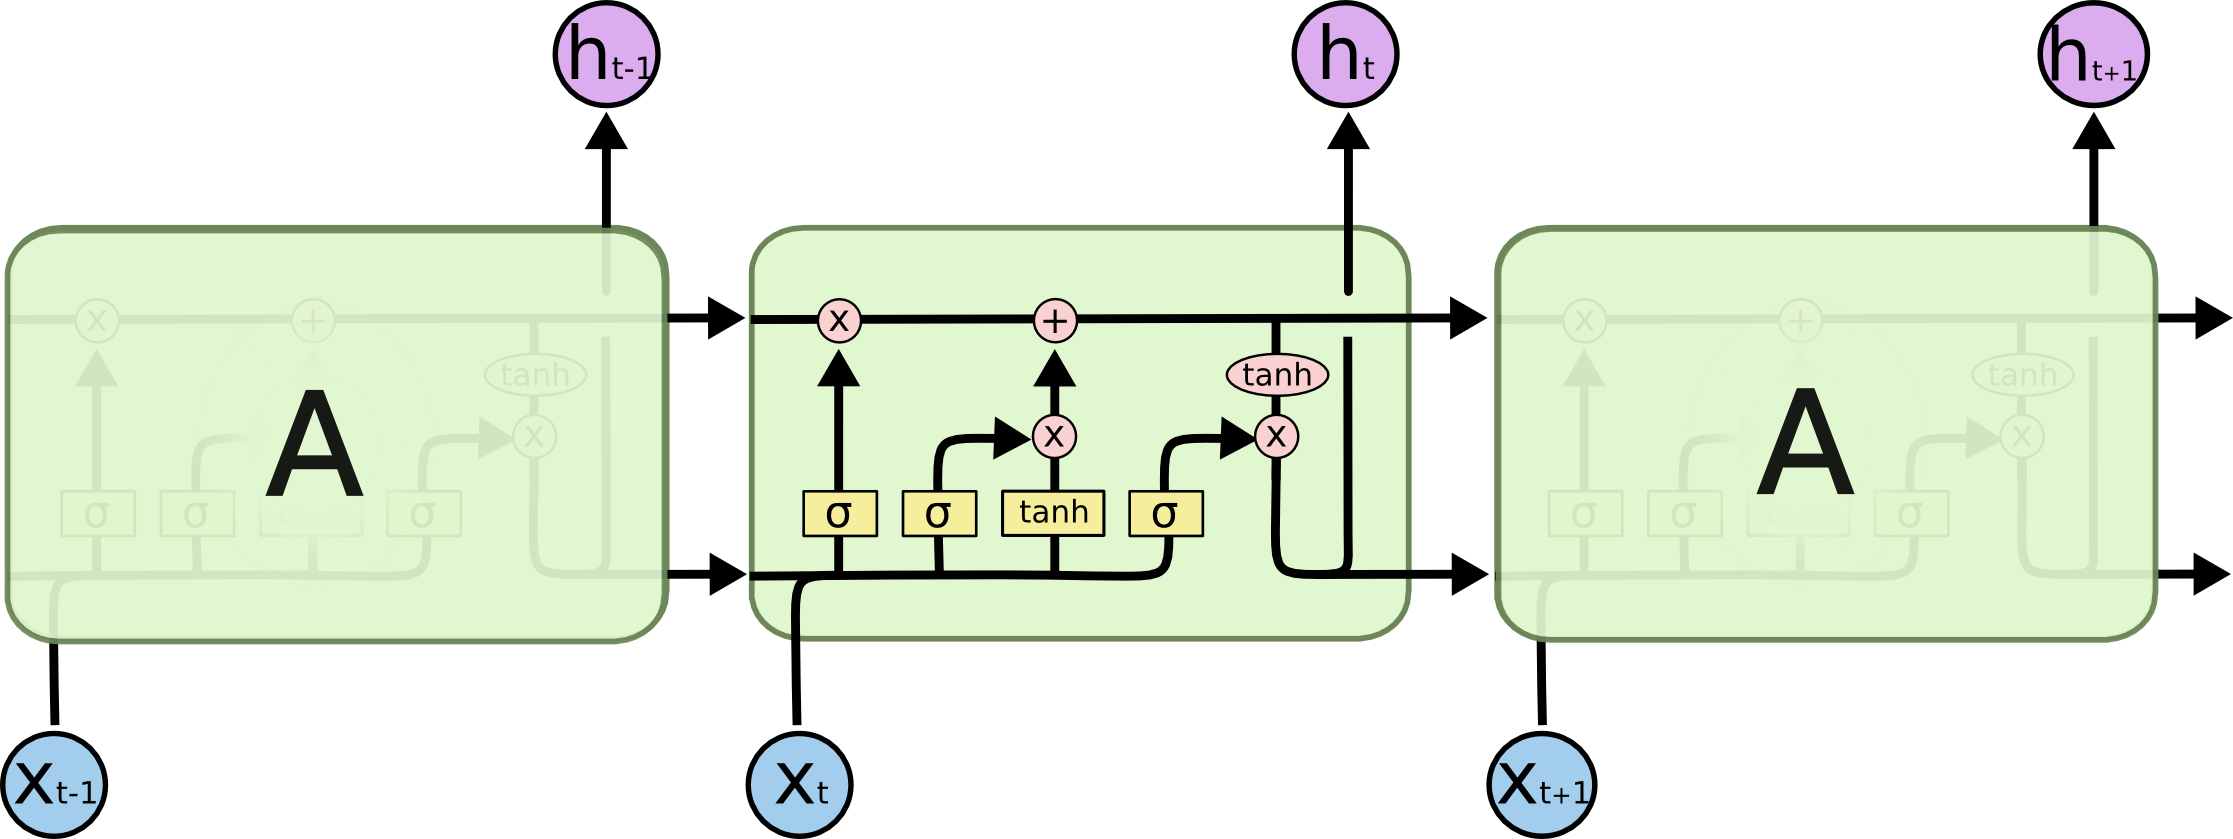
\includegraphics[width=\columnwidth]{figures/LSTM3-chain.png}
	\caption{Struttura di una cella LSTM. \textit{fonte:} \cite{lstmblog} }
\label{fig:lstm}
\end{figure}

\subsection{Output Encoder}
L'output in uscita da questo encoder è in forma di un tensore monodimensionale, di dimensione fissata, contenente le caratteristiche principali che compongono un nome di dominio.

\section{Decoder}
La struttura del decoder è lascamente una copia speculare dell'encoder. L'obiettivo principale è riuscire a ricampionare un dominio partendo da un tensore a domensione inferiore rispetto alla codifica fornita in input all'encoder.

La struttura di massima presenta come primo layer un \textit{repeat vector} che ripete il tensore di input per un numero di volte pari alla lunghezza massima di dominio, fissata in fase di codifica del dataset, formando così un tensore 3-dimensionale, dello stessa dimensione dei domini provenienti dal dataset. La sequenza così formata viene data in input ad un layer LSTM avente le identiche caratteristiche del layer LSTM presente all'interno dell'encoder. Successivamente la sequenza di emissioni in output dalla LSTM viene fornita ad due reti convoluzionali parallele identiche al quelle inserite all'interno dell'encoder. il risultato di tale operazione è un vettore di dimensione pari a dizionario di caratteri ammissibili per i domini, per ogni step della sequenza di caratteri che compone un dominio. In Figura \ref{fig:decoder} viene mostrato lo schema di massima del \textit{decoder}.

\begin{figure}[!htb]
    \centering
	%\documentclass{standalone}
%\usepackage{tikz}
%
%\usetikzlibrary{shapes,arrows,fit,calc,positioning}
%\usetikzlibrary{backgrounds}
\tikzstyle{box} = [draw, rectangle, fill=white, rounded corners, thick, node distance=5em, text width=7em, text centered, minimum height=2.5em]
\tikzstyle{container} = [draw, rectangle, dashed, inner sep=1em, node distance=5em]
\tikzstyle{line} = [draw, thick, -latex']
%\begin{document}
\begin{tikzpicture}[auto]
	\node [box] (conv) {Convolution Layer};
%	\node [box, below of=conv] (batch) {Batch Normalization};
%	\node [box, below of=batch](leaky) {Leaky ReLU activation};
%	\node [box, below of=leaky](dropout) {Dropout};
	\node [box, below of=conv](pooling){Average Pooling};

	\node [box, right of=conv, node distance=12em] (conv2) {Convolution Layer};
%	\node [box, below of=conv2] (batch2) {Batch Normalization};
%	\node [box, below of=batch2](leaky2) {Leaky ReLU activation};
%	\node [box, below of=leaky2](dropout2) {Dropout};
	\node [box, below of=conv2](pooling2){Average Pooling};
	
	\node [draw=none, above of=conv](invis4){};
	\node [draw=none, above of=conv2](invis5){};
	\node [draw=none, fit=(invis4)(invis5)](invis6){};
	\coordinate[above of=invis6,node distance=3em](begin_enc);
	\coordinate[above of=begin_enc,node distance=3em](in);
	\node at (begin_enc.north) [above,node distance=0 and 0] (input){};
	\node at (in.north) [box] (lstm){LSTM};	
	\node [box, above of=lstm](repvec){Repeat Vector};
	\coordinate [above of=repvec, node distance=3em](in);
	\node at (in.north)[above, node distance=0 and 0](testo_in){Dominio Codificato};	
	
	\node [draw=none, below of=pooling](invis){};
	\node [draw=none, below of=pooling2](invis2){};
	\node [draw=none, fit=(invis)(invis2)](invis3){};
	
	\node[box,below of=invis3, node distance=3em](conc){Concatenation Layer};
	\node[box,below of=conc](regr){Multinomial Regression};
	\coordinate[below of=regr,node distance=3em](end_enc);
	\node at (end_enc.south) [below,node distance=0 and 0] (output){Dominio};
	
	% area tratteggiata
	\node [container, fit=(conv)(pooling)](cnn){};
	\node [container, fit=(conv2)(pooling2)](cnn2){};
	\node at (cnn.north west) [above right,node distance=0 and 0] {Convnet};
	\node at (cnn2.north east) [above left,node distance=0 and 0] {Convnet};
	%%%%

	%%% frecce
	\path [line] (conv) -- (pooling);
%	\path [line] (batch) -- (leaky);
%	\path [line] (leaky) -- (dropout);
%	\path [line] (dropout) -- (pooling);
	\path [line] (pooling) |- (conc);

	\path [line] (conv2) -- (pooling2);
%	\path [line] (batch2) -- (leaky2);
%	\path [line] (leaky2) -- (dropout2);
%	\path [line] (dropout2) -- (pooling2);
	\path [line] (pooling2) |- (conc);
	
	\path [line] (conc) -- (regr);
	\path [line] (regr) -- (end_enc);
	
	\path [line] (in) -- (repvec);
	\path [line] (repvec) -- (lstm);
	\draw (lstm) -- (begin_enc);
	\path [line] (begin_enc) -| (conv);
	\path [line] (begin_enc) -| (conv2);
\end{tikzpicture}
%\end{document}
	\caption{Struttura dell'\textit{decoder}}
\label{fig:decoder}
\end{figure}

\subsection{Regressione Multinomiale}
Lo step finale del decoder è un livello \textit{dense} di tipo \textit{time-distributed} che agisce come \textit{regressore multinomiale}, in grado di eseguire classificazione in diverse classi (in questo caso una classe per ogni carattere possibile nel dizionario). Il regressore multinomiale utilizza un tipo di attivazione \textit{softmax}, definito dalla funzione:

\[\sigma(\mathbf{z})_j = \frac{e^{z_j}}{\sum_{k=1}^K e^{z_k}}\qquad  \text{per}\; j=1,\ldots,K. \] 

dove $k$ è la dimensione del vettore di input $\mathbf{z}$ mentre in uscita si ottiene un vettore $k$-dimensionale $\sigma(\mathbf{z})$ di valori compresi in un intervallo $\left(0,1\right)$. Grazie a tale attivazione sull'ultimo layer, l'output del decoder rappresenta una distribuzione multinomiale rispetto ai caratteri di ammissibili, per ogni step temporale che compone. 
Tale distribuzione può essere campionata in modo da ottenere di nuovo un vettore numerico di interi contenente i caratteri codificati all'interno del vocabolario di caratteri ammissibili per i domini. 

Per il campionamento è stato usata una funzione \textit{softmax} utilizzata nel campo dell'apprendimento per rinforzo \cite{reinflearning}, definita come: 

\[P_t(a) = \frac{\exp(q_t(a)/\tau)}{\sum_{i=1}^n\exp(q_t(i)/\tau)} \text{,}\]

Dove il valore di\textit{ "azione"} $q_{t}(a)$ corrisponde alla "ricompensa" ottenuta per l'azione $a$ e $\tau$  è definito come parametro di \textit{"temperatura"}. Per alte \textit{"temperature"} ( $\tau \to \infty$ ), tutte le azioni hanno la stessa probabilità e più bassa la temperatura, più la "ricompensa" influisce sulla probabilità. Per basse tempeature ($\tau \to 0^{+}$), la probabilità di \textit{azione} con la ricompensa più alta tende ad 1. 

Tramite questa funzione è stato possibile mettere a a punto in fase sperimentale il campionamento dei domini dalla lo rappresentazione in forma di tensore alla rappresentazione testuale.

\section{Generative Adversarial Network}
\label{ganintro}
La \textit{Generative Adversarial Network (abbr. GAN)} èun modello di rete neurale formata da due reti che competono l'una contro l'altra: un \textit{generatore} che cerca di creare dati sintetici basati sulla vera distribuzione, con l'aggiunta di rumore in input ed un \textit{discriminatore}, che riceve un campione e deve predire se appartiene al set reale o sintetico. Questo processo continua in forma di competizione tra le due reti, nella quale il discriminatore apprende in maniera sempre più accurata a distinguere i campioni ed il generatore apprende la costruzione di dati sintetici sempre più realistici. In figura \ref{fig:gan} si può vedere una struttura di massima di una GAN.

Il seguente step di lavoro è stato trasformare l'autoencoder definito a partire dalla sezione \ref{autoencoder} in una GAN.
\begin{figure}[!htb]
    \centering
	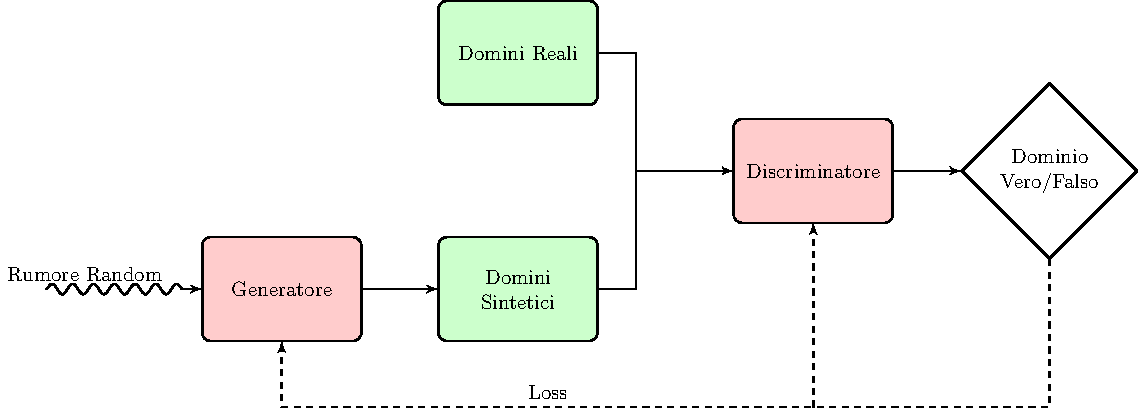
\includegraphics[width=0.9\columnwidth]{figures/gan.tex}
	\caption{Struttura di una \textit{Generative Adversarial Network}}
\label{fig:gan}
\end{figure}


\subsection{Architettura GAN}
\label{ganarch}

\todo{schema GAN preso da autoencoder}

\todo{parlare della semplificazione della GAN rispetto al paper deepDGA}

\chapter{Implementazione}
\label{implementazione}


\section{Classificatore Random Forest}
\label{imp:randomforest}

\section{Classificatore Neurale}
\label{imp:classneurale}

\section{Autoencoder}
\label{imp:autoencoder}

\section{Generative Adversarial Network}
\label{imp:gan}

\todo{parlare del pretraining}
\chapter{Risultati}
In questo capitolo si presentano i risultati della fase sperimentale effettuata su tutti i sistemi mostrati precedentemente: classificatore \textit{random forest}, classificatore neurale, autoencoder e GAN. Le metriche di valutazione utilizzate sono enunciate all'interno della sezione \ref{metriche}. In sezione \ref{res:crf} vengono mostrati i risultati sperimentali ottenuti dal classificatore random forest, punto di partenza di questo studio. In sezione \ref{ris:cnn} vengono mostrati i risulati sperimentali ottenuti dal classificatore neurale, evoluzione del classificatore random forest, e le problematiche incontrate durante tale fase. In sezione \ref{ris:autoenc} viene mostrata la fase sperimentale che ha coinvolto l'autoencoder, per durante la quale si sono ottenuti i pesi utilizzati successivamente come punto di partenza per la fase di training della Generative Adversarial Network. All'interno dell'ultima sezione ( \ref{ris:gan} ) sono mostrati i risultati ottenuti dal training della GAN e la lunga fase di tuning richiesta da quest'ultima.

\pagebreak
\section{Metriche di valutazione}
\label{metriche}
Le metriche di valutazione utilizzate per testare la qualità dei modelli sono state:
\begin{itemize}
\item \textbf{Precision}: il rapporto $\frac{t_p}{t_p+f_p}$ dove $t_p$ è il numero di veri positivi e $f_p$ il numero di falsi positivi. Intuitivamente è l'abilità del classificatore di non marcare come positivo un campione negativo.
\item \textbf{Recall}: il rapporto $\frac{t_p}{t_p+f_n}$  dove $f_n$ sono i falsi negativi. Intuitivamente è l'abilità del classificatore di trovare tutti i campioni positivi.
\item \textbf{F-score}: è definito come la media armonica tra \textit{precision} e \textit{recall}: 
\[F_1 = 2 \cdot \frac{1}{\tfrac{1}{\mathrm{recall}} + \tfrac{1}{\mathrm{precision}}} = 2 \cdot \frac{\mathrm{precision} \cdot \mathrm{recall}}{\mathrm{precision} + \mathrm{recall}}\]
\item \textbf{Area sottesa da Receiver Operating Characteristic}:  metodo grafico per la valutazione della qualità di un classificatore binario al variare della soglia di discriminazione. E' creata graficando la frazione dei veri positivi rispetto ai campioni positivi ($tpr$ = True positive rate) contro la frazione dei falsi positivi rispetto ai campioni negativi ($fpr$ = False positive rate). L'area sottesa dalla curva ROC equivale alla probabilità che il classificatore predica un campione positivo casuale rispetto ad un campione negativo casuale. Formalmente è definita da:
\[ A = \int_{\infty}^{-\infty} \mbox{TPR}(T) \left(-\mbox{FPR}'(T)\right) \, dT = \int_{-\infty}^{\infty} \int_{-\infty}^{\infty} I(T'>T)f_1(T') f_0(T) \, dT' \, dT = P(X_1 > X_0)\]
dove 
$X_{1}$ è il punteggio per un'istanza positiva e $X_{0}$ è il punteggio per un'istanza negativa, mentre $f_{0}$ e $f_{1}$ sono densità di probabilità che un campione sia negativo ($1$) o positivo ($0$)
\end{itemize}

\newpage
\section{Classificatore Supervisionato}
\label{res:crf}
Il classificatore Random Forest è stato testato in diverse configurazioni. La configurazione che è stata presentata nella sezione \ref{imp:randomforest} ha mostrato i migliori risultati in ogni test.

Il classificatore è stato testato dapprima testato con le seguenti famiglie di malware, contro un subset di dimensione simile di domini provenienti dalla classifica Alexa.

\begin{table}[!bp]
    \centering
    \begin{tabular}[t]{l}
    \toprule
    Malware Families \\
    \midrule
	legit \\
	cryptolocker \\
	zeus \\
	pushdo \\
	rovnix \\
	tinba \\
	conficker \\
	matsnu \\
	ramdo \\
	\bottomrule
\end{tabular}
\caption{\label{tab:malware}}
\end{table}

Il dataset così riunito è stato separato in due parti disuguali: il 90\% è stato utilizzato come dataset di training mentre il restante 10\% come testing in maniera da evitare il fenomeno di overfitting. I risultati della predizione sul dataset di testing sono mostrati in figura \ref{fig:repdga} e figura \ref{fig:rocdga}. A fianco dell'etichette \textit{legit} e \textit{DGA} è indicato il numero di campioni utilizzati per le due categorie. Come si può notare la performance del classificatore è molto positiva. Si ipotizza che tale risultato sia dovuto alla forte differenza linguistica tra domini reali e domini DGA, pertanto il classificatore soffre di un errore praticamente nullo. 

\begin{figure}[htbp]
    \centering
    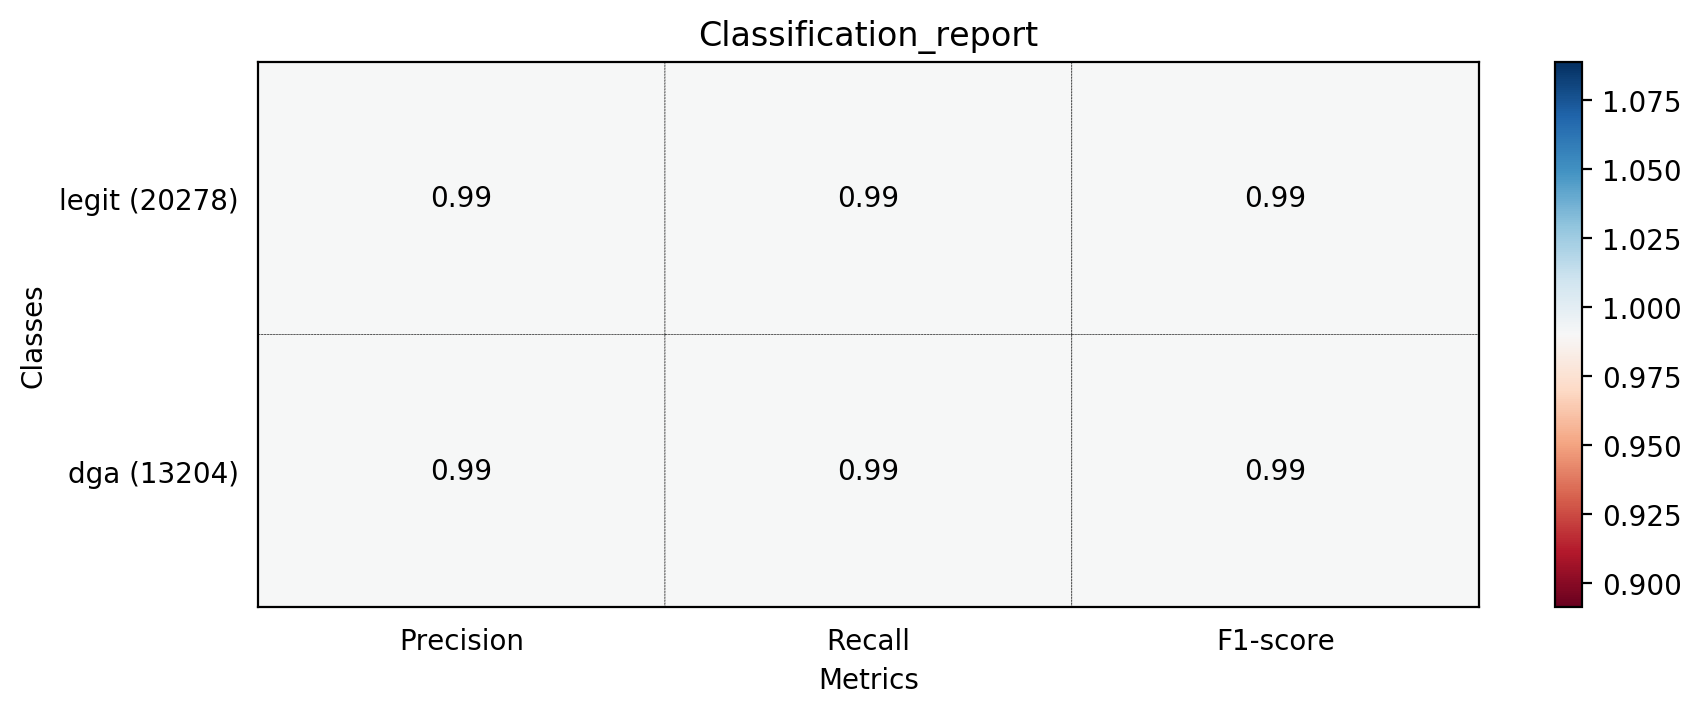
\includegraphics[width=.85\columnwidth]{figures/rndf_tra_nosup_nosup/class_rep.png}
    \caption{Classificatore Random Forest: Report di classificazione su un subset di domini reali (legit) e malevoli (DGA).\label{fig:repdga}}

    \centering
    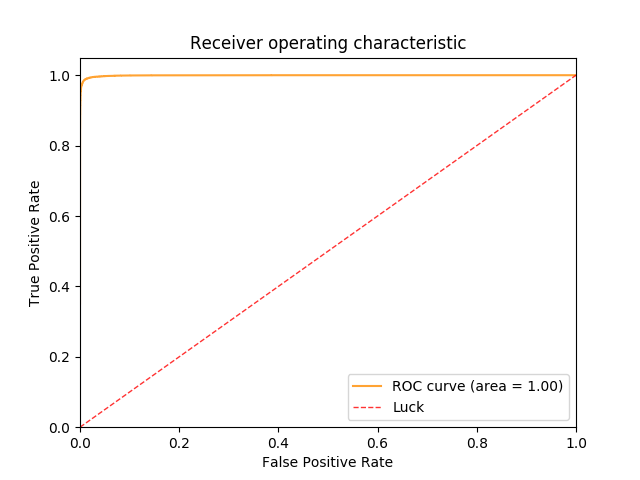
\includegraphics[width=.85\columnwidth]{figures/rndf_tra_nosup_nosup/roc_plot.png}
    \caption{Classificatore Random Forest: Area sottesa dalla curva ROC per il test con domini di tabella \ref{tab:malware}.\label{fig:rocdga}}
\end{figure}

In fase preliminare si è effettuato un confronto con altri due algoritmi di classificazione: SVC (C-Support Vector) e Gaussian Naive-Bayes. La loro performance non è stata altrettanto eccellente e pertanto si è deciso di accantonarli e proseguire con l'utilizzo di Random Forest. I report di classificazione sono mostrati in figura \ref{fig:repsvc} e \ref{fig:repgnb}.

\begin{figure}[htbp]
  	\centering
    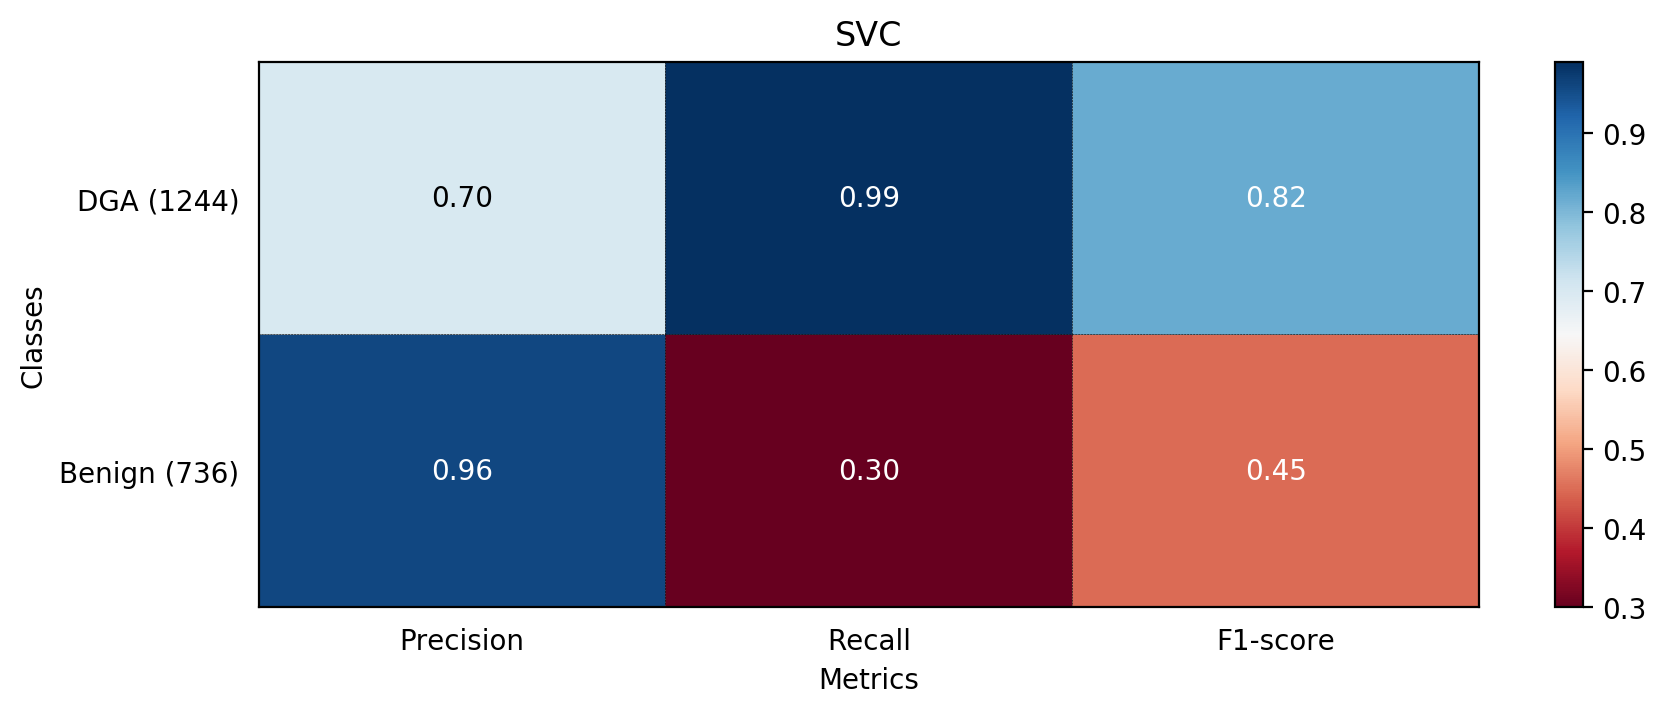
\includegraphics[width=.85\columnwidth]{figures/report_SVC.png}
    \caption{Report di classificazione per l'algoritmo SVC.\label{fig:repsvc}}

	\centering
    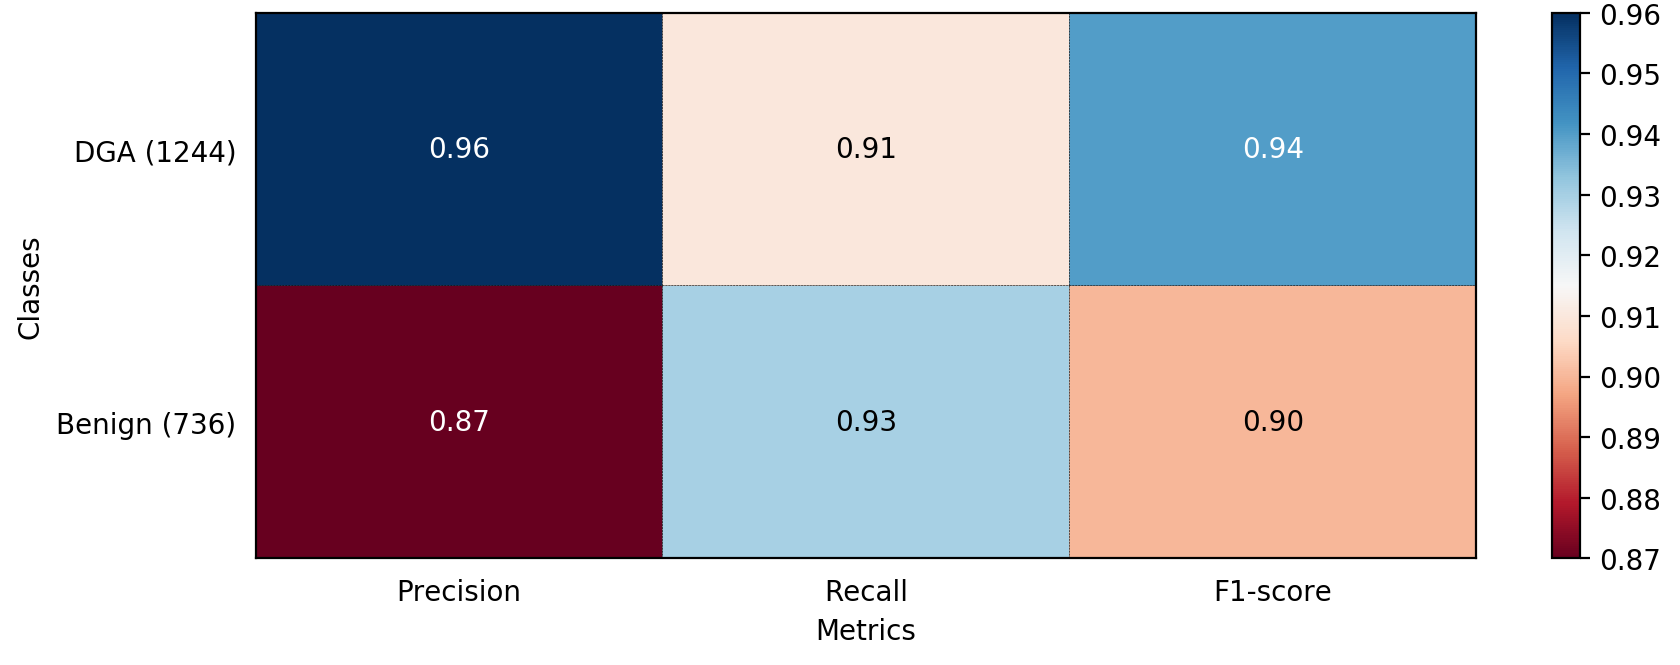
\includegraphics[width=.85\columnwidth]{figures/report_GaussianNB.png}
    \caption{Report di classificazione per l'algoritmo Gaussian Naive-Bayes.\label{fig:repgnb}}
\end{figure}

Il classificatore random forest è stato testato inserendo \textit{suppobox} tra le famiglie DGA già presenti. Si è scelto tale malware come campione esterno in quanto presenta la maggiore differenza rispetto alle famiglie mostrate in tabella \ref{tab:malware}. I risultati si possono vedere in figura \ref{fig:repsup} e \ref{fig:rocsup} e come si può notare la performance ne è fortemente influenzata, introducendo una grande percentuale di falsi nelle predizioni effettuate dal classificatore.

\begin{figure}[!bp]
    \centering
    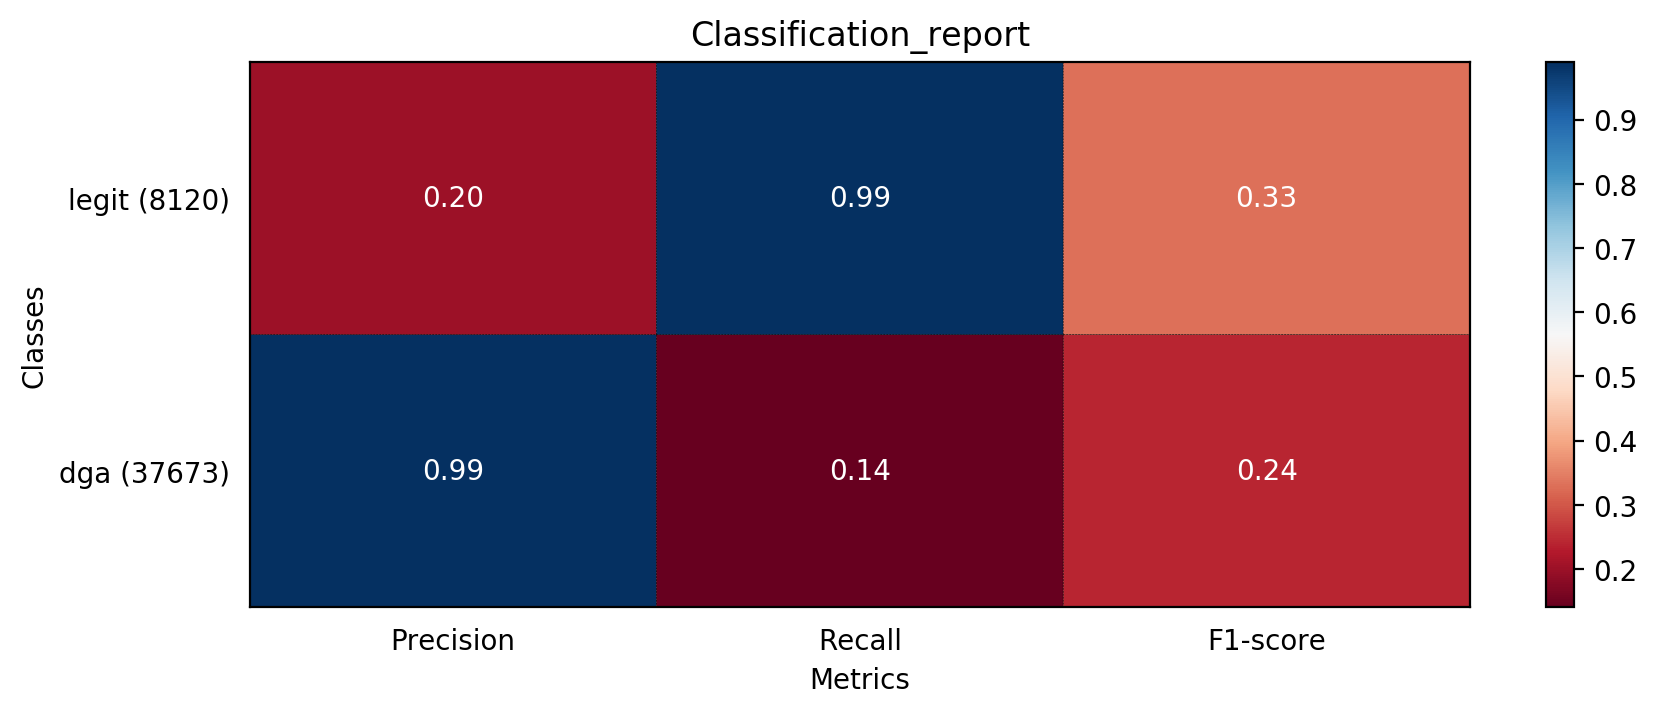
\includegraphics[width=.85\columnwidth]{figures/rndf_tra_nosup_sup/class_rep.png}
    \caption{Classificatore Random Forest: Report di classificazione su un subset di domini reali (legit) e malware, comprendenti suppobox (DGA).\label{fig:repsup}}

    \centering
    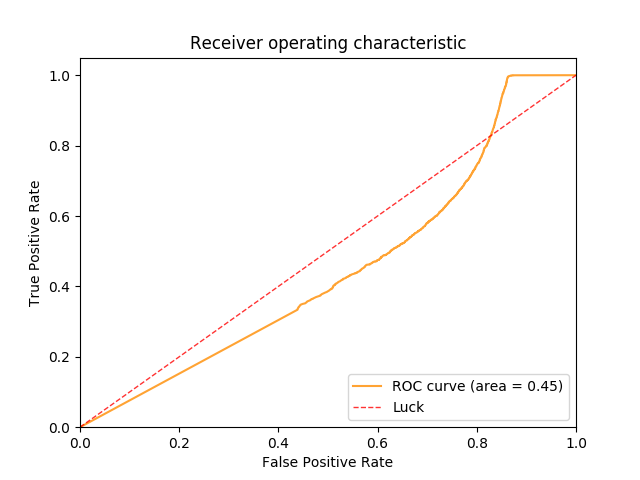
\includegraphics[width=.85\columnwidth]{figures/rndf_tra_nosup_sup/roc_plot.png}
    \caption{Classificatore Random Forest: Area sottesa dalla curva ROC per il test con  suppobox.\label{fig:rocsup}}
\end{figure}

\newpage
Come ultimo test è stato eseguito il training aggiungendo al precedente dataset di training una parte di domini generati da suppobox (Figura \ref{fig:repall} e \ref{fig:rocall}). Come si può notare la performance è migliorata sensibilmente, non raggiungendo comunque i risultati eccellenti del primo test.

\begin{figure}[!bp]
    \centering
    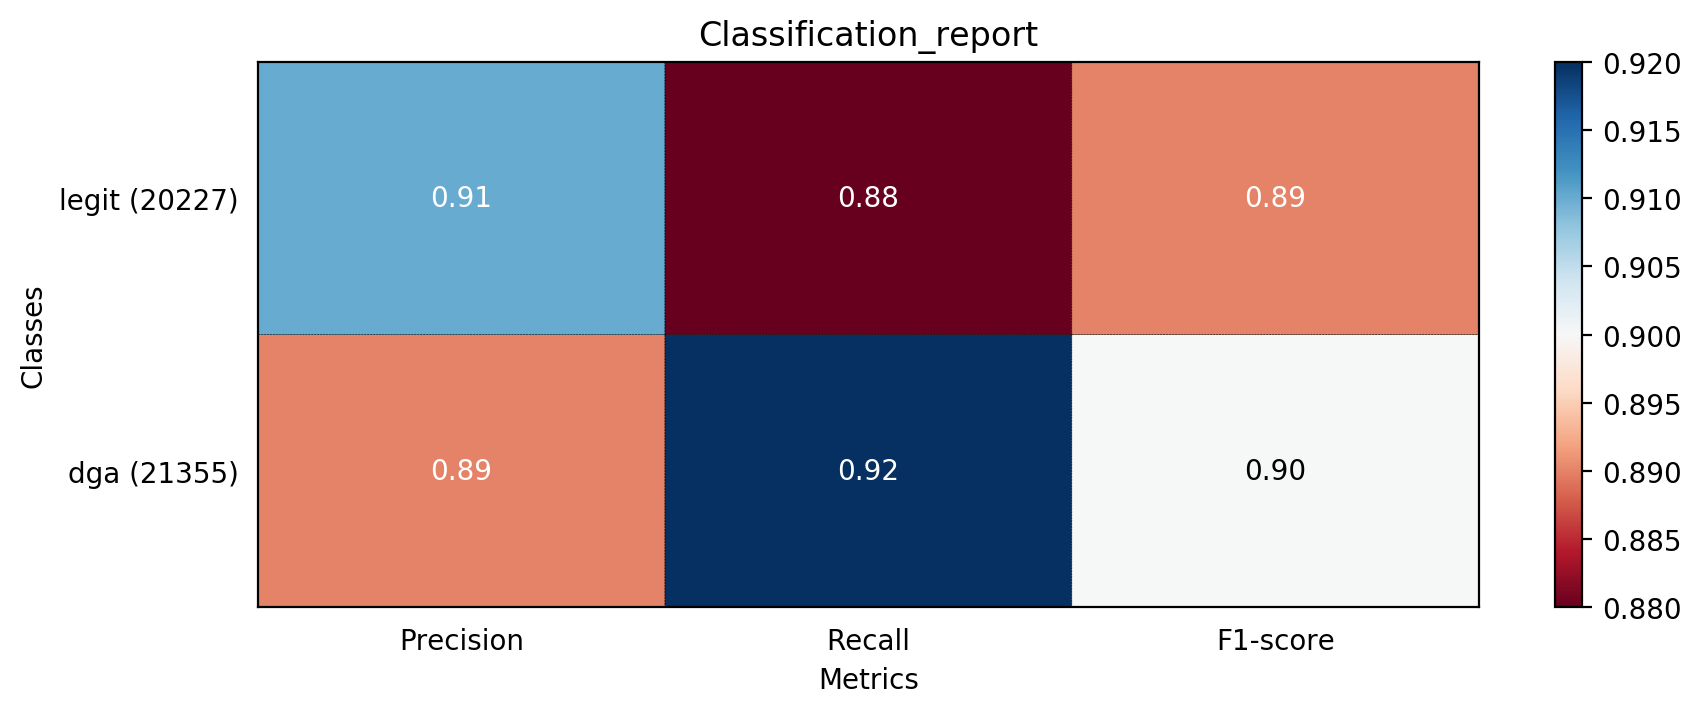
\includegraphics[width=.85\columnwidth]{figures/rndf_tra_sup_sup/class_rep.png}
    \caption{Classificatore Random Forest: Report di classificazione su un subset di domini reali (legit) e malware, comprendenti suppobox (DGA).\label{fig:repall}}

    \centering
    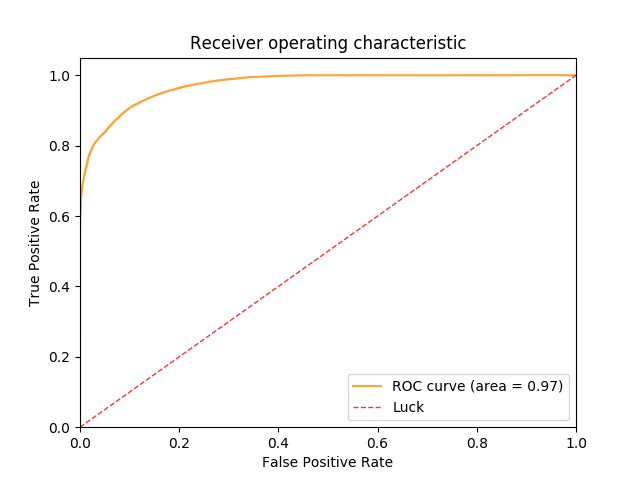
\includegraphics[width=.85\columnwidth]{figures/rndf_tra_sup_sup/roc_plot.png}
    \caption{Classificatore Random Forest: Area sottesa dalla curva ROC per il test con domini reali e malware (comprendenti suppobox).\label{fig:rocall}}
\end{figure}

\newpage
\section{Classificatore Neurale}
\label{ris:cnn}
Il classificatore neurale, nato per superare le mancanze del classificatore random forest, è stato testato nelle stesse condizioni utilizzate precedentemente: in particolare è stato utilizzato lo stesso dataset mostrato in sezione \ref{res:crf} e diviso ancora una volta in $\frac{9}{10}$ per la fase di training e $\frac{1}{10}$ per la fase di testing.

In prima fase si sono messe a confronto le tre architetture presentate in sezione \ref{classificatorenninterno}. Tali architetture hanno dimostrato tre andamenti simili; tuttavia a fronte dei risultati mostrati e della minore richiesta di risorse, il modello intermedio è risultato vincente rispetto agli altri testati. ( Figura \ref{fig:cfrmlp} )


\todo{parlarne nella fase implementativa}

\begin{figure}[!bp] 
\centering
	\begin{minipage}[t]{\linewidth}
		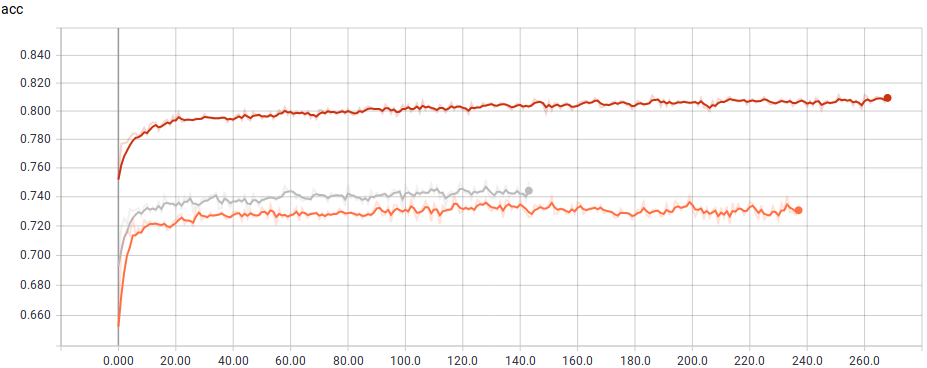
\includegraphics[width=\linewidth]{figures/MLP1.png}
	\end{minipage}\hfill
	\begin{minipage}[b]{\linewidth}
		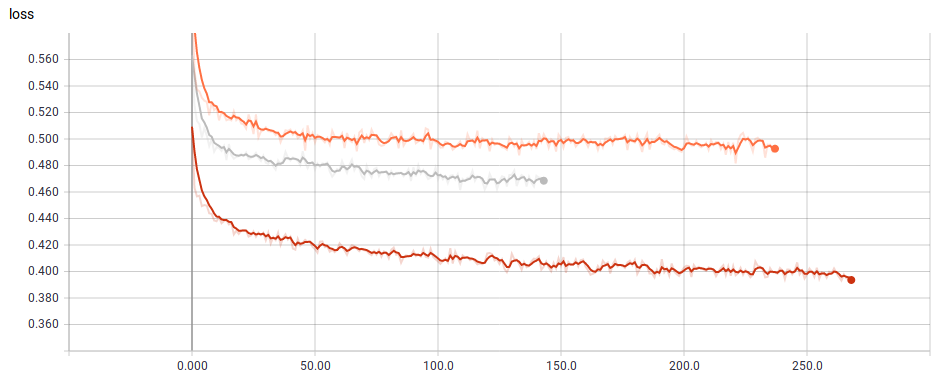
\includegraphics[width=\linewidth]{figures/MLP2.png}
	\end{minipage}
	\caption{Classificatore Neurale: Grafici di Accuracy e Loss  in funzione del tempo. confronto fra i tre modelli. La curva di colore grigio rappresenta il modello ingrandito, la curva di colore arancione rappresenta il modello ridotto mentre la curva di colore rosso rappresenta il modello intermedio; vincente tra i tre. \label{fig:cfrmlp}}
\end{figure}

Motivo di confronto è stata l'introduzione o meno di Batch Normalization \cite{1502.03167}. Come si può vedere dai grafici mostrati in figura \ref{fig:batchnorm} vi è una differenza di prestazione dovuta alla normalizzazione dei mini-batch, pertanto si è scelto di mantenere tale funzione all'interno dei livelli nonostante l'aumento di costi prestazionali.

\begin{figure}[!bp] 
	\begin{minipage}[t]{\linewidth}
		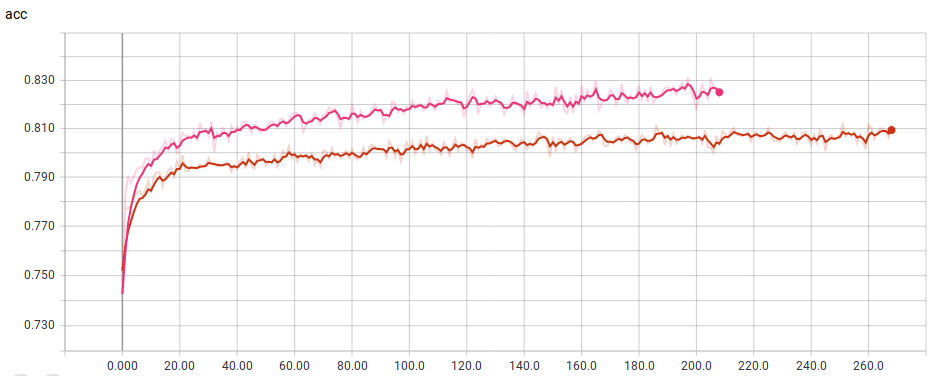
\includegraphics[width=\linewidth]{figures/MLP_batchnorm1.png}
	\end{minipage}\hfill
	\begin{minipage}[b]{\linewidth}
		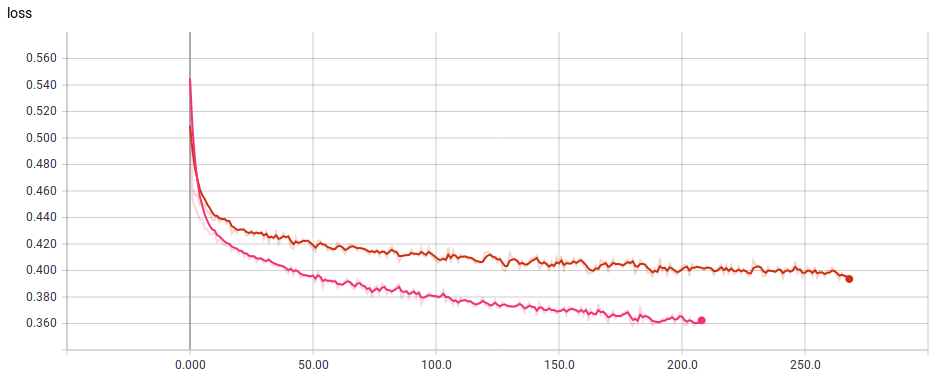
\includegraphics[width=\linewidth]{figures/MLP_batchnorm2.png}
	\end{minipage}
	\caption{Classificatore Neurale: Grafici di Accuracy e Loss in funzione del tempo per il modello intermedio. La curva rossa identifica il modello senza l'ausilio di Batch Normalization mentre la curva fuchsia rappresenta lo stesso modello con l'inserimento di Batch Normalization per ogni livello densamente connesso che compone il Multilayer Perceptron. \label{fig:batchnorm}}
\end{figure}

Particolarmente difficoltoso si è dimostrato il tuning degli  iperparametri di numero epoche e dimensione mini-batch per ottenere valori ottimali. Dopo una serie di test sperimentali che hanno messo a confronto diversi valori, si sono rilevati i valori
\begin{itemize}
\item \textbf{numero epoche} $= 60$
\item \textbf{dimensione minibatch} $= 35$ 
\end{itemize}

Tali valori hanno dimostrato di fornire la migliore performance durante la fase di training.

I test effettuati sul dataset hanno mostrato i risultati mostrati in figura \ref{fig:cnrepall} e \ref{fig:cnrocall}. Come si può vedere dai grafici il comportamento del classificatore è pressoché identico a quello mostrato dal classificatore random forest (figure \ref{fig:repall} e \ref{fig:rocall} )

\begin{figure}[!bp]
    \centering
    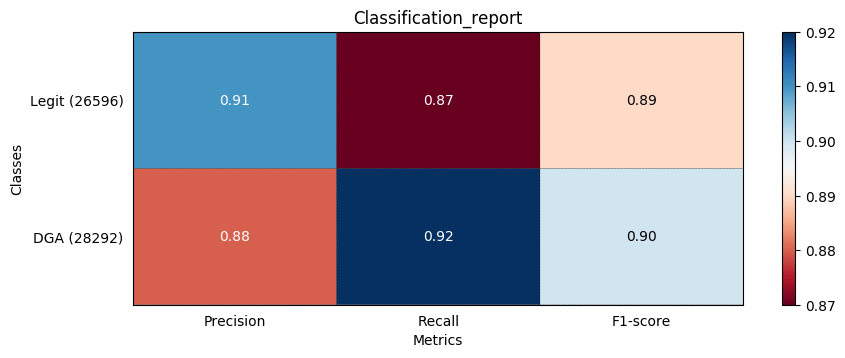
\includegraphics[width=.85\columnwidth]{figures/clas_nn/class_rep.png}
    \caption{Classificatore Neurale: Report di classificazione su un subset di domini reali (legit) e malware, comprendenti suppobox (DGA).\label{fig:cnrepall}}

    \centering
    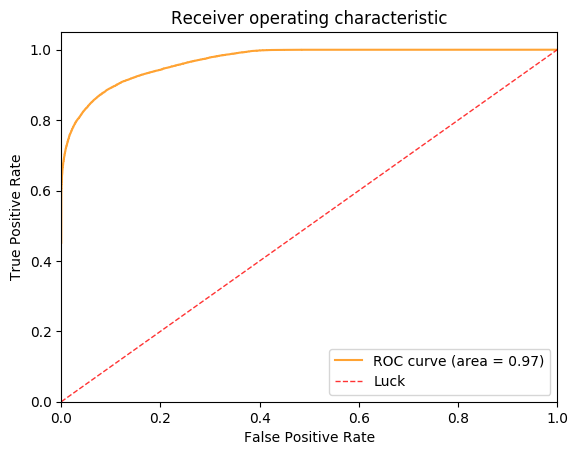
\includegraphics[width=.85\columnwidth]{figures/clas_nn/roc_plot.png}
    \caption{Classificatore Neurale: Area sottesa dalla curva ROC per il test con domini reali e malware (comprendenti suppobox).\label{fig:cnrocall}}
\end{figure}

A partire da questo classificatore neurale stabile è stato possibile implementare un sistema di adversarial learning tramite la GAN derivante da un autoencoder. 

\newpage
\section{Autoencoder}
\label{ris:autoenc}
L'autoencoder come presentato in sezione \ref{autoencoder} è stato testato con il dataset mostrato in sezione \ref{imp:autoencoder:dataset}. In fase sperimentale si è proceduto alla quantificazione della configurazione ottimale dell'autoencoder. In particolare si sono messi a confronto i valori di dropout presenti all'interno di encoder e decoder ed i valori di learning rate dei rispettivi compilatori. I valori finali di tali compilatori sono indicati all'interno della sezione \ref{imp:autoe:enc} e \ref{imp:autoe:dec}

In figura \ref{fig:aut1} e \ref{fig:aut2} è possibile notare i risultati della fase di training, per il quale si è trattenuto $\frac{1}{3}$ del training set come subset di validazione. Come è possibile notare l'ultima iterazione (colore verde) ha mostrato i risultati migliori e pertanto è stata utilizzata come base di partenza per il training della successiva GAN. 

L'utilizzo dei pesi dell'autoencoder come punto di partenza per il training della GAN ha contribuito fortemente a ridurre la instabilità di tale sistema, permettendo ai due sottosistemi generatore e discriminatore di partire da predizioni più precise rispetto all'utilizzo di pesi inizializzati in maniera randomica come generalmente attuato.

In tabella \ref{tab:autoenc} è possibile vedere un esempio di quali domini l'autoencoder produce dato un subset del dataset Alexa in input. Si può notare come siano vagamente simili ai domini reali per quanto riguarda la distribuzione dei caratteri e la lunghezza media dei domini, tuttavia non presenta ulteriori caratteristiche tali da influenzare negativamente i classificatori neurali.

\begin{table}[!hbp]
\centering
	\begin{tabular}{l}
	\toprule
	ehyt5tcncn3o5nw \\
	reknclkobg \\
	kne3xersl6npyr5 \\
	moeaamutlrhsn \\
	5t7-iitnvtrm5en \\
	r-zeotn0t-wuf \\
	bgargtas \\
	vviadammpielw \\
	7-aolelcfiextl \\
	morehekb \\
	\bottomrule
	\end{tabular}
	\begin{tabular}{l}
	\toprule
	d9ongedeo  \\
	meoomer \\
	zggy1lbxgi1psir \\
	ypsanilwrox \\
	bt5ennsl1zjchp0 \\
	runvpfcfrmaser \\
	anhgnxracokimoa \\
	atngsam \\
	de-poaz9yiiu \\
	nhntadt \\
	\bottomrule
	\end{tabular}
	\begin{tabular}{l}
	\toprule
	2kbth \\
	snd-drcepn \\
	sievd0 \\
	ono5ponlanafhic \\
	mmd0-5-ile \\
	su1aojp52 \\
	eraveok \\
	lfeubune \\
	ilnegban0 \\
	uim-rca0ohxmsbi \\
	\bottomrule
	\end{tabular}
	\begin{tabular}{l}
	\toprule
	oldohizlioczzu \\
	dodttiune \\
	ahoinin3 \\
	etiso9oo \\
	qi8gtuyte-ssg-n \\
	mlsrp8gf \\
	ktb1r2vb \\
	ptsdrqtanflog \\
	mcng5tsotnless \\
	rrhtsrceu \\
	\bottomrule
	\end{tabular}

\caption{Esempio di domini generati dall'autoencoder. \label{tab:autoenc}}
\end{table}

\begin{figure}[p]
    \centering
    \begin{minipage}[t]{0.7\linewidth}
    	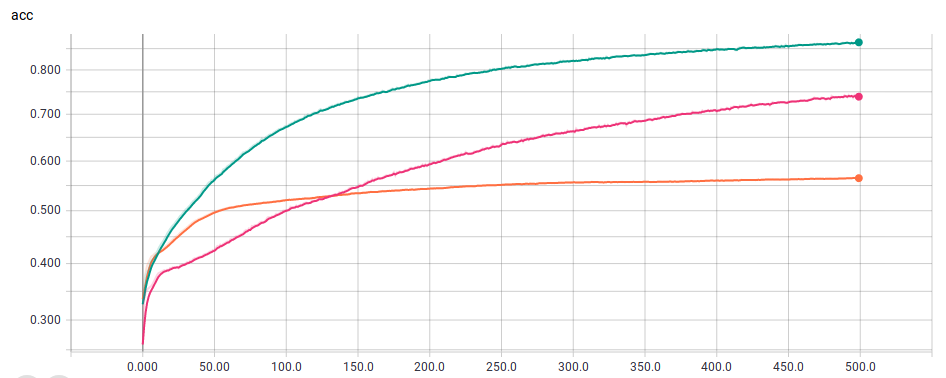
\includegraphics[width=\linewidth]{figures/autoenc.png}
    \end{minipage}\hfill
    \begin{minipage}[b]{0.7\linewidth}
    	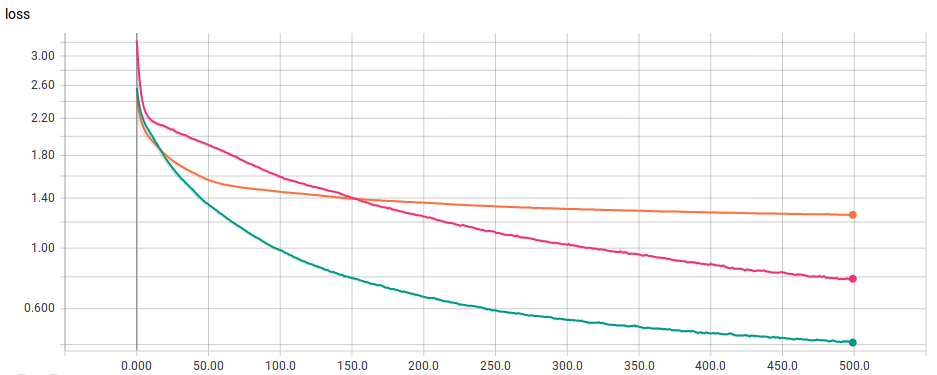
\includegraphics[width=\linewidth]{figures/autoenc2.png}
    \end{minipage}
    \caption{Grafici di Accuracy e Loss in funzione del tempo per la fase di training dell'autoencoder. La prima fase è rappresentata dalla curva arancione, la seconda dalla curva fuchsia mentre la terza fase è rappresentata dalla curva di colore verde. Si può notare come la terza iterazione raggiunga buoni valori di accuracy e loss; pertanto stato scelto come configurazione vincente per la GAN \label{fig:aut1}}
\end{figure}

\begin{figure}[p]
    \centering
    \begin{minipage}[t]{0.7\linewidth}
    	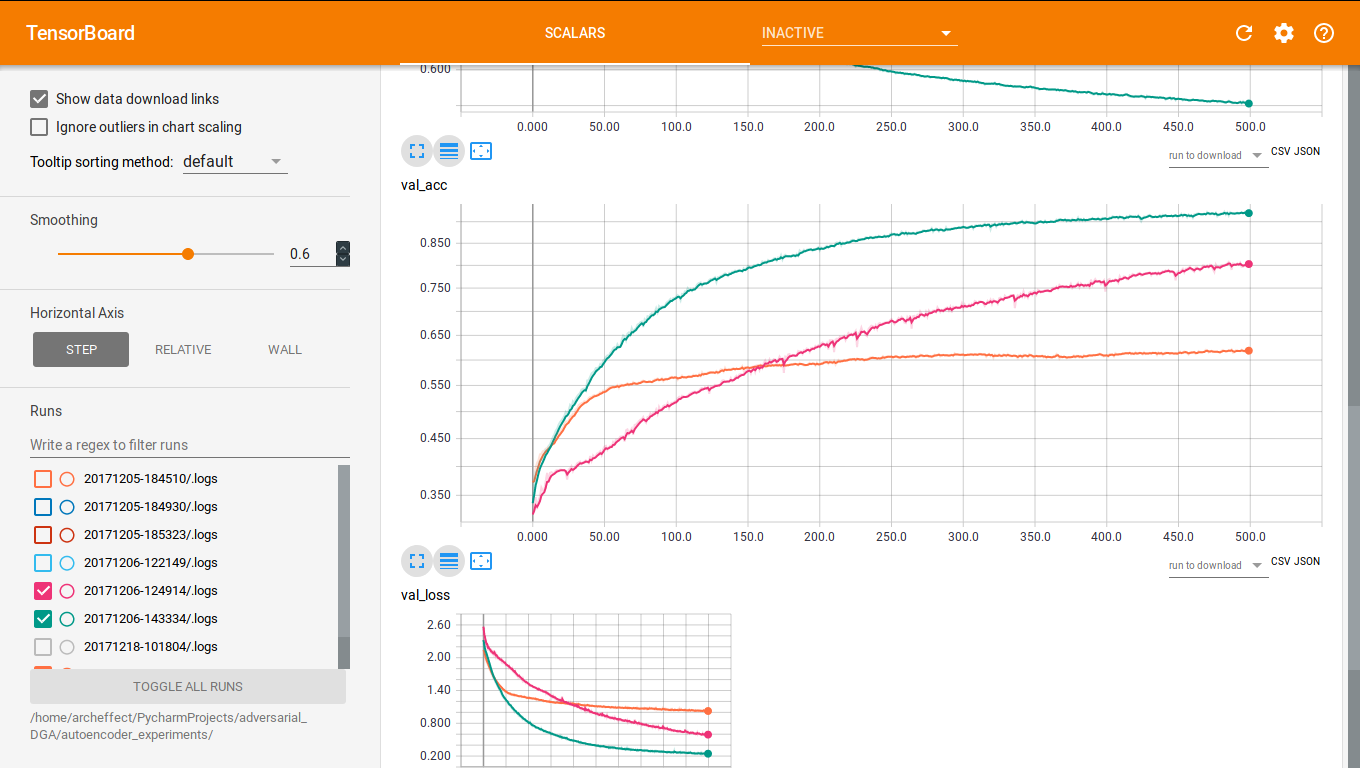
\includegraphics[width=\linewidth]{figures/autoenc3.png}
    \end{minipage}\hfill
    \begin{minipage}[b]{0.7\linewidth}
    	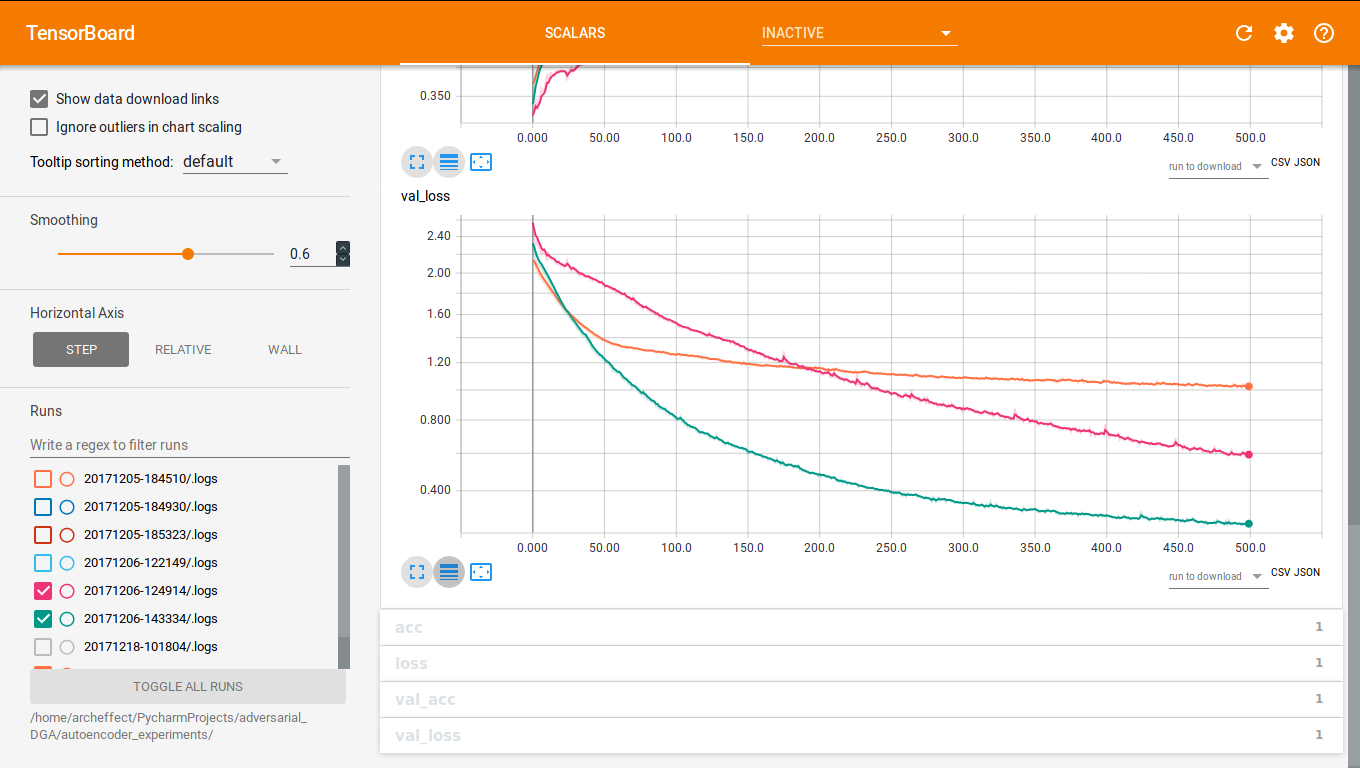
\includegraphics[width=\linewidth]{figures/autoenc4.png}
    \end{minipage}
    
\caption{Grafici di Accuracy e Loss in funzione del tempo rispetto al subset di validazione per la fase di training dell'autoencoder. Si può notare come i valori raggiunti siano molto simili a quelli ottenuti sul dataset di training, indice di qualità del modello rispetto a valori mai visti. \label{fig:aut2} }
\end{figure}

\newpage
\section{Generative Adversarial Network}
\label{ris:gan}
La Generative Adversarial Network descritta in sezione \ref{ganintro} e implementata come in sezione \ref{imp:gan} ha richiesto una lunga fase sperimentale nella quale è stato necessario trovare la giusta combinazione di iperparametri per i quali i due sottosistemi generatore e discriminatore potessero rimanere in equilibrio durante la durata necessaria per completare la fase di training. 

In particolare si sono incontrati due \textit{failure modes}:
\begin{itemize}
\item Caso in cui il discriminatore prevale sul generatore, come mostrato in figura \ref{fig:ganfailure1}, si ottiene una curva di \textit{loss} rasente lo zero, causando al generatore un incremento costante della propria curva di loss. Il significato di tale comportamento è l'impossibilità del generatore di generare domini sintetici sufficientemente realistici da poter mettere in crisi la predizione del discriminatore.
\item Caso in cui il generatore degeneri, producendo "spazzatura", rendendo eccessivamente semplice la predizione del discriminatore. La degenerazione infatti avviene in forma di domini generati tutti uguali, contenente una singola lettera ripetuta per tutta la lunghezza di caratteri. Tale comportamento è dovuto alla mancata capacità del generatore di mimare realisticamente i domini realistici. Un esempio di tale comportamento è mostrato in figura \ref{fig:ganfailure2}
\end{itemize}

\begin{figure}[!bp]
    \centering
    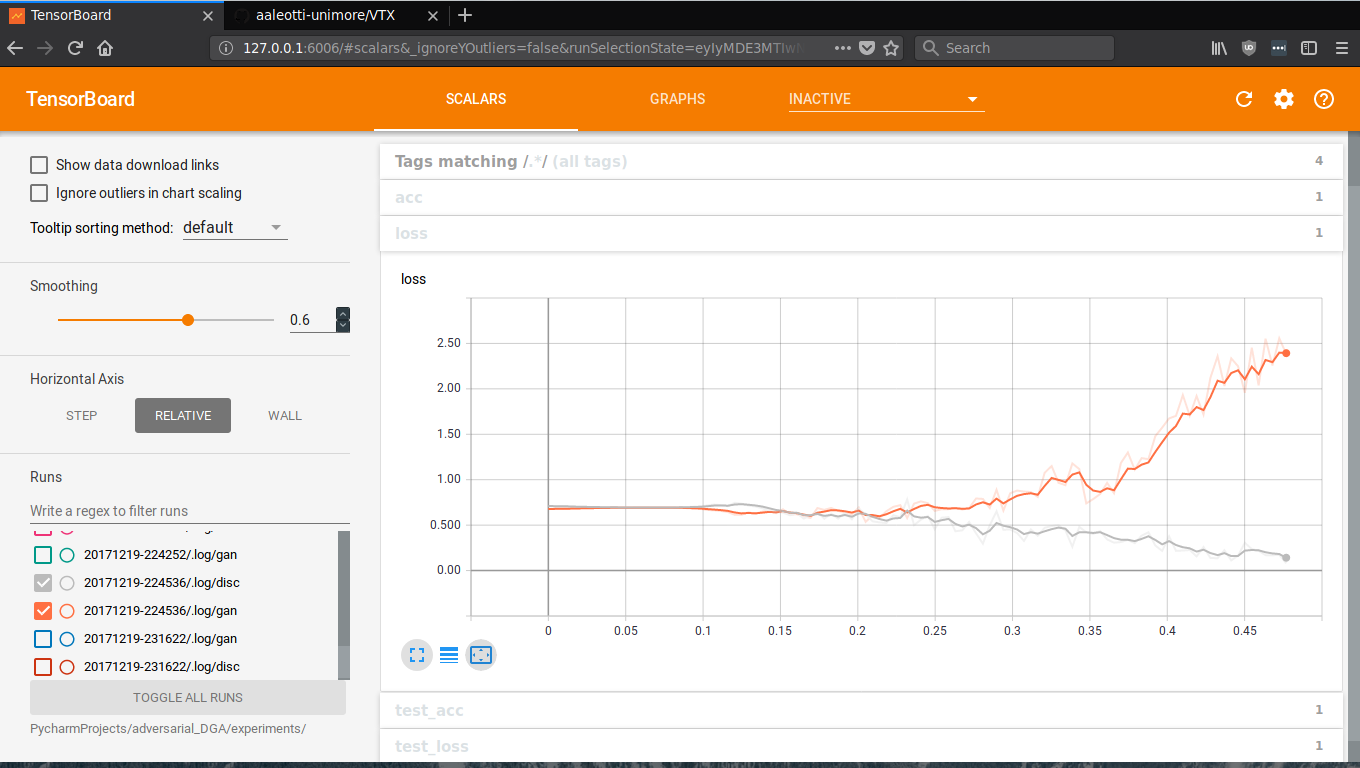
\includegraphics[width=\columnwidth]{figures/gan/ganfailure1.png}
    \caption{Caso di degenerazione 1. Grafico del valore di loss in funzione del tempo. Il discriminatore (curva di colore grigio) prevale sul generatore (curva arancione), il quale non riesce a migliorare il proprio valore di loss.\label{fig:ganfailure1}}

    \centering
    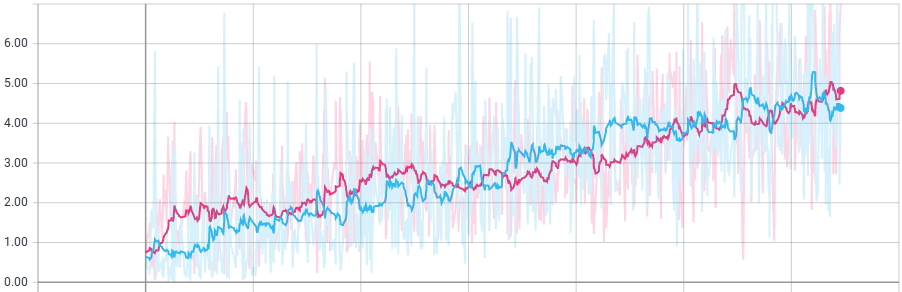
\includegraphics[width=\columnwidth]{figures/gan/ganfailure2.png}
    \caption{Caso di degenerazione 2. Grafico del valore di loss in funzione del tempo. Il generatore (curva di colore azzurro) non produce domini realistici, degenerando a dati inutilizzabili. Il discriminatore (curva di colore rosso) di conseguenza migliora la propria loss a causa della differenza sempre maggiore tra domini realistici e domini sintetici. \label{fig:ganfailure2}}
\end{figure}

E' stato possibile ottenere la stabilità della GAN, grazie a numerose tecniche empiriche ottenute da \cite{1606.03498} ed all'utilizzo del pre-training fornendo come inizializzazione i pesi ottenuti dalla fase di training dall'autoencoder. In figura \ref{fig:ganok} si può vedere l'andamento dei valori di loss di generatore e discriminatore nel caso di equilibrio tra le due reti neurali.

\begin{figure}[!bp]
\centering
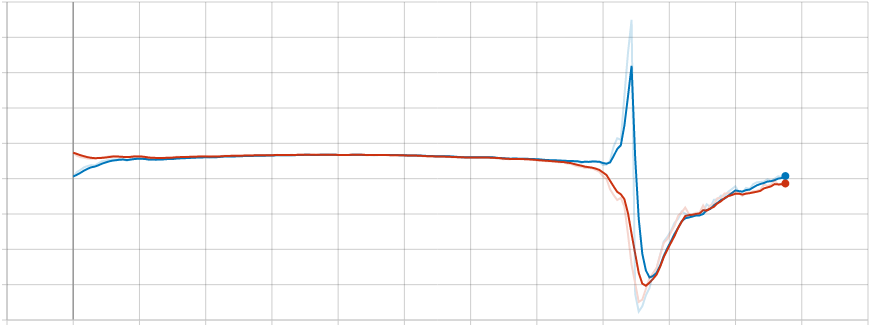
\includegraphics[width=\columnwidth]{figures/gan/ganok.png}
\caption{Grafico di loss in funzione del tempo per discriminatore (curva di colore rosso) e generatore (curva di colore azzurro). L'andamento rimane equilibrato fino al punto in cui il generatore non riesce a generare nuovi domini in grado di mettere in crisi il discriminatore. \label{fig:ganok}}
\end{figure}

Grazie a tale training è stato possibile infine generare un dataset di domini sintetici provenienti dalla GAN, che mimassero in maniera più precisa i domini realistici. Come si può notare in tabella \ref{tab:gan} non si tratta di una rappresentazione di parole realmente esistenti, tuttavia si può notare come siano presenti n-grammi realmente esistenti oltre che ad una lunghezza di sequenza simile a domini reali.

\begin{table}[!bp]
\centering
	\begin{tabular}{l}
	\toprule
edarareve \\
skonasesosarere \\
skaran-unar \\
chicochophavock \\
dichoros \\
isherevores \\
nillersosersrsp \\
rldicde \\
escrarararuro \\
aemjtup \\
	\bottomrule
	\end{tabular}
	\begin{tabular}{l}
	\toprule
	ssrarsone \\
asccacca \\
monasheamc \\
itsusosose \\
stlega \\
ivortewrp \\
sdesedlsss \\
nggeneneres \\
madesadk \\
cesasasrrrrrrs \\
	\bottomrule
	\end{tabular}
	\begin{tabular}{l}
	\toprule
	horicicocr \\
sthonacorl \\
raocjcacarcrarl \\
vichitos \\
ogagagasuss \\
plerundinwoshn \\
odocococcocke \\
tuccronpcs \\
mivorthitdhud \\
mtuvocaro \\
	\bottomrule
	\end{tabular}
	\begin{tabular}{l}
	\toprule
avensdends \\
mwonwonerene \\
inihkkellgcrock \\
madoxto \\
ljarlers \\
maahofononoris \\
msusongere \\
scsacccca \\
rrngajiagjonggk \\
ituutasisa \\
	\bottomrule
	\end{tabular}

\caption{Esempio di domini generati dalla GAN. \label{tab:gan}}
\end{table}

Come si può notare dal confronto mostrato in figura \ref{fig:chardistr} la distribuzione dei caratteri generata dalla GAN è molto simile a quella presente all'interno del dataset Alexa, dimostrando la natura dei domini sintetici rispetto a quelli reali.
Il classificatore neurale presentato nelle sezioni precedenti è stato messo alla prova utilizzando un subset circa 10000 domini generati dalla GAN, etichettati come DGA, ed un subset di 10000 domini reali provenienti dal dataset Alexa. Come si può vedere da figura \ref{fig:repgan} il classificatore si trova in grave difficoltà nel distinguere i domini sintetici, raggiungendo un bassissimo valore di recall, l'abilità di riconoscere i campioni positivi forniti. Lo score medio del classificatore ne risulta molto basso  rispetto a quello precedentemente mostrato in figura \ref{fig:cnrepall}. In figura \ref{fig:rocgan} è mostrata la curva ROC del classificatore neurale testato nelle medesime condizioni: la ridottissima area sottesa  ( $ AUC = 0.39$ ) dimostra come il classificatore non sia in grado di distinguere in maniera efficiente i domini reali da quelli generati dalla GAN. 

Tali risultati a confronto con quelli mostrati in sezione \ref{res:crf} e \ref{ris:cnn} dimostrano come i domini sintetici generati dalla GAN siano in grado di influenzare negativamente la performance di un classificatore DGA che in precedenza ha dimostrato buoni risultati.

\begin{figure}[!bp]
    \centering
    \begin{minipage}[t]{0.45\columnwidth}
		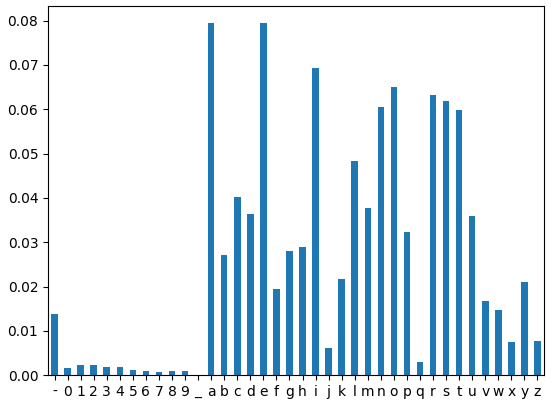
\includegraphics[width=\linewidth]{figures/all_legit_char_distr.png}
	\end{minipage}
	\begin{minipage}[b]{0.45\columnwidth}
		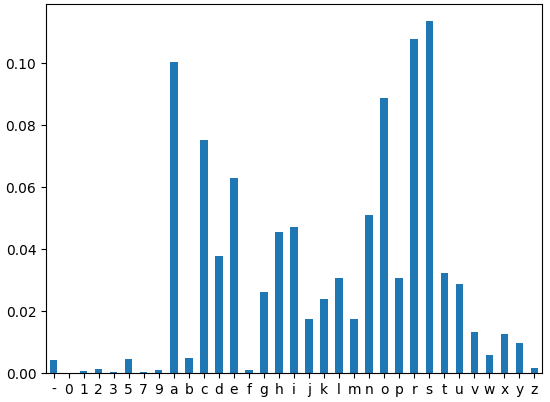
\includegraphics[width=\linewidth]{figures/chars_histogram.png}
	\end{minipage}
\caption{Confronto della distribuzione dei caratteri reali (grafico a sinistra) e generati algoritmicamente dalla GAN (grafico a destra) \label{fig:chardistr}}
\end{figure}

\begin{figure}[p]
    \centering
    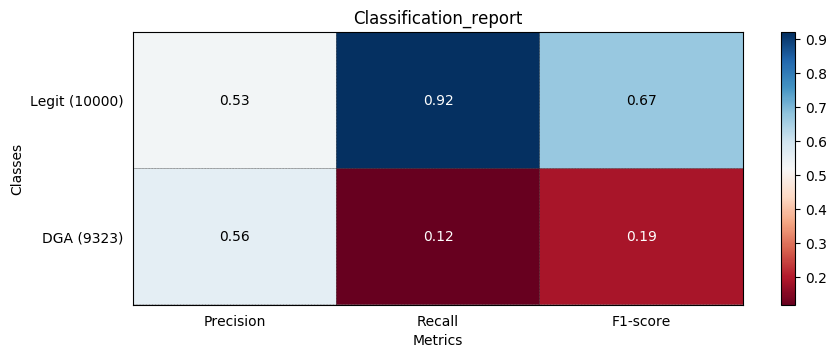
\includegraphics[width=\columnwidth]{figures/gan/class_rep.png}
    \caption{Classificatore Neurale testato su GAN: Report di classificazione su un subset di domini reali (legit) e generati da GAN (DGA).\label{fig:repgan}}

    \centering
    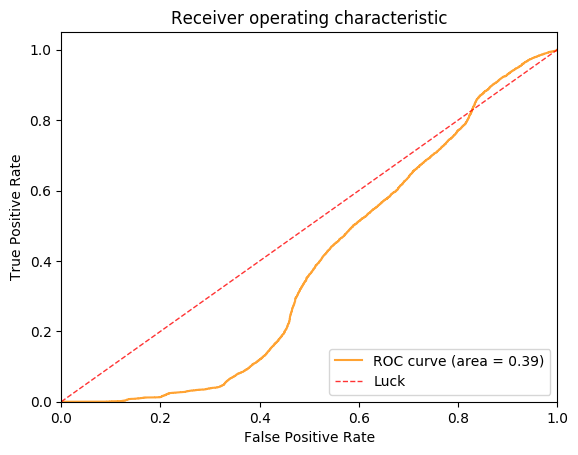
\includegraphics[width=\columnwidth]{figures/gan/roc_plot.png}
    \caption{Classificatore Random Forest: Area sottesa dalla curva ROC per il test con domini reali e generati da GAN.\label{fig:rocgan}}
\end{figure}

\chapter{Conclusioni}
\label{conclusioni}

In questo capitolo si propongono degli esempi per gli oggetti utilizzati più di frequente in latex: la Sezione~\ref{citazioni} descrive come scrivere citazioni, la Sezione~\ref{oggetti-float} propone degli esempi di oggetti float, la Sezione~\ref{compilazione} descrive come compilare questo documento.



% PAGINA VUOTA
%\clearpage\null\thispagestyle{empty}\clearpage
%\appendix
%\appendixpage
%\addappheadtotoc

%\clearpage\null\thispagestyle{empty}\clearpage


%\listoffigures


\begin{flushleft}
\bibliographystyle{ieeetr}
\bibliography{sections/references} 
\end{flushleft}

\end{document}
